%%
%% Beginning of file 'sample62.tex'
%%
%% Modified 2018 January
%%
%% This is a sample manuscript marked up using the
%% AASTeX v6.2 LaTeX 2e macros.
%%
%% AASTeX is now based on Alexey Vikhlinin's emulateapj.cls 
%% (Copyright 2000-2015).  See the classfile for details.

%% AASTeX requires revtex4-1.cls (http://publish.aps.org/revtex4/) and
%% other external packages (latexsym, graphicx, amssymb, longtable, and epsf).
%% All of these external packages should already be present in the modern TeX 
%% distributions.  If not they can also be obtained at www.ctan.org.

%% The first piece of markup in an AASTeX v6.x document is the \documentclass
%% command. LaTeX will ignore any data that comes before this command. The 
%% documentclass can take an optional argument to modify the output style.
%% The command below calls the preprint style  which will produce a tightly 
%% typeset, one-column, single-spaced document.  It is the default and thus
%% does not need to be explicitly stated.
%%
%%
%% using aastex version 6.2
\documentclass[preprint2]{aastex62}
\usepackage{amsmath}
\usepackage{microtype}
\usepackage{bm}
\usepackage{dsfont}
\usepackage{listings}
\usepackage{url}
\usepackage{tikz}
\usetikzlibrary{shapes,arrows}
\usepackage{natbib}
\lstset{
	basicstyle=\ttfamily,
	mathescape,
}
%% The default is a single spaced, 10 point font, single spaced article.
%% There are 5 other style options available via an optional argument. They
%% can be envoked like this:
%%
%% \documentclass[argument]{aastex62}
%% 
%% where the layout options are:
%%
%%  twocolumn   : two text columns, 10 point font, single spaced article.
%%                This is the most compact and represent the final published
%%                derived PDF copy of the accepted manuscript from the publisher
%%  manuscript  : one text column, 12 point font, double spaced article.
%%  preprint    : one text column, 12 point font, single spaced article.  
%%  preprint2   : two text columns, 12 point font, single spaced article.
%%  modern      : a stylish, single text column, 12 point font, article with
%% 		  wider left and right margins. This uses the Daniel
%% 		  Foreman-Mackey and David Hogg design.
%%  RNAAS       : Preferred style for Research Notes which are by design 
%%                lacking an abstract and brief. DO NOT use \begin{abstract}
%%                and \end{abstract} with this style.
%%
%% Note that you can submit to the AAS Journals in any of these 6 styles.
%%
%% There are other optional arguments one can envoke to allow other stylistic
%% actions. The available options are:
%%
%%  astrosymb    : Loads Astrosymb font and define \astrocommands. 
%%  tighten      : Makes baselineskip slightly smaller, only works with 
%%                 the twocolumn substyle.
%%  times        : uses times font instead of the default
%%  linenumbers  : turn on lineno package.
%%  trackchanges : required to see the revision mark up and print its output
%%  longauthor   : Do not use the more compressed footnote style (default) for 
%%                 the author/collaboration/affiliations. Instead print all
%%                 affiliation information after each name. Creates a much
%%                 long author list but may be desirable for short author papers
%%
%% these can be used in any combination, e.g.
%%
%% \documentclass[twocolumn,linenumbers,trackchanges]{aastex62}
%%
%% AASTeX v6.* now includes \hyperref support. While we have built in specific
%% defaults into the classfile you can manually override them with the
%% \hypersetup command. For example,
%%
%%\hypersetup{linkcolor=red,citecolor=green,filecolor=cyan,urlcolor=magenta}
%%
%% will change the color of the internal links to red, the links to the
%% bibliography to green, the file links to cyan, and the external links to
%% magenta. Additional information on \hyperref options can be found here:
%% https://www.tug.org/applications/hyperref/manual.html#x1-40003
%%
%% If you want to create your own macros, you can do so
%% using \newcommand. Your macros should appear before
%% the \begin{document} command.
%%
\newcommand{\vdag}{(v)^\dagger}
\newcommand\aastex{AAS\TeX}
\newcommand\latex{La\TeX}
\newcommand{\thickbar}[1]{\mathbf{\bar{\text{$#1$}}}}
%% Tells LaTeX to search for image files in the 
%% current directory as well as in the figures/ folder.
\graphicspath{{./}{figures/}}

%% Reintroduced the \received and \accepted commands from AASTeX v5.2
%\received{January 1, 2018}
%\revised{January 7, 2018}
%\accepted{\today}
%% Command to document which AAS Journal the manuscript was submitted to.
%% Adds "Submitted to " the arguement.
%\submitjournal{ApJ}

%% Mark up commands to limit the number of authors on the front page.
%% Note that in AASTeX v6.2 a \collaboration call (see below) counts as
%% an author in this case.
%
%\AuthorCollaborationLimit=3
%
%% Will only show Schwarz, Muench and "the AAS Journals Data Scientist 
%% collaboration" on the front page of this example manuscript.
%%
%% Note that all of the author will be shown in the published article.
%% This feature is meant to be used prior to acceptance to make the
%% front end of a long author article more manageable. Please do not use
%% this functionality for manuscripts with less than 20 authors. Conversely,
%% please do use this when the number of authors exceeds 40.
%%
%% Use \allauthors at the manuscript end to show the full author list.
%% This command should only be used with \AuthorCollaborationLimit is used.

%% The following command can be used to set the latex table counters.  It
%% is needed in this document because it uses a mix of latex tabular and
%% AASTeX deluxetables.  In general it should not be needed.
%\setcounter{table}{1}

%%%%%%%%%%%%%%%%%%%%%%%%%%%%%%%%%%%%%%%%%%%%%%%%%%%%%%%%%%%%%%%%%%%%%%%%%%%%%%%%
%%
%% The following section outlines numerous optional output that
%% can be displayed in the front matter or as running meta-data.
%%
%% If you wish, you may supply running head information, although
%% this information may be modified by the editorial offices.
\shorttitle{JUPITER Data Processing}
\shortauthors{Nasedkin}
%%
%% You can add a light gray and diagonal water-mark to the first page 
%% with this command:
% \watermark{text}
%% where "text", e.g. DRAFT, is the text to appear.  If the text is 
%% long you can control the water-mark size with:
%  \setwatermarkfontsize{dimension}
%% where dimension is any recognized LaTeX dimension, e.g. pt, in, etc.
%%
%%%%%%%%%%%%%%%%%%%%%%%%%%%%%%%%%%%%%%%%%%%%%%%%%%%%%%%%%%%%%%%%%%%%%%%%%%%%%%%%

%% This is the end of the preamble.  Indicate the beginning of the
%% manuscript itself with \begin{document}.
\tikzstyle{block} = [rectangle, draw, fill=white, text width=5em, text centered,  minimum height=2em]
\tikzstyle{line} = [draw, -latex']
\begin{document}


\title{Processing JUPITER Hydrodynamics Simulation Data for Visualisation in Paraview.}

%% LaTeX will automatically break titles if they run longer than
%% one line. However, you may use \\ to force a line break if
%% you desire. In v6.2 you can include a footnote in the title.

%% A significant change from earlier AASTEX versions is in the structure for 
%% calling author and affilations. The change was necessary to implement 
%% autoindexing of affilations which prior was a manual process that could 
%% easily be tedious in large author manuscripts.
%%
%% The \author command is the same as before except it now takes an optional
%% arguement which is the 16 digit ORCID. The syntax is:
%% \author[xxxx-xxxx-xxxx-xxxx]{Author Name}
%%
%% This will hyperlink the author name to the author's ORCID page. Note that
%% during compilation, LaTeX will do some limited checking of the format of
%% the ID to make sure it is valid.
%%
%% Use \affiliation for affiliation information. The old \affil is now aliased
%% to \affiliation. AASTeX v6.2 will automatically index these in the header.
%% When a duplicate is found its index will be the same as its previous entry.
%%
%% Note that \altaffilmark and \altaffiltext have been removed and thus 
%% can not be used to document secondary affiliations. If they are used latex
%% will issue a specific error message and quit. Please use multiple 
%% \affiliation calls for to document more than one affiliation.
%%
%% The new \altaffiliation can be used to indicate some secondary information
%% such as fellowships. This command produces a non-numeric footnote that is
%% set away from the numeric \affiliation footnotes.  NOTE that if an
%% \altaffiliation command is used it must come BEFORE the \affiliation call,
%% right after the \author command, in order to place the footnotes in
%% the proper location.
%%
%% Use \email to set provide email addresses. Each \email will appear on its
%% own line so you can put multiple email address in one \email call. A new
%% \correspondingauthor command is available in V6.2 to identify the
%% corresponding author of the manuscript. It is the author's responsibility
%% to make sure this name is also in the author list.
%%
%% While authors can be grouped inside the same \author and \affiliation
%% commands it is better to have a single author for each. This allows for
%% one to exploit all the new benefits and should make book-keeping easier.
%%
%% If done correctly the peer review system will be able to
%% automatically put the author and affiliation information from the manuscript
%% and save the corresponding author the trouble of entering it by hand.

\correspondingauthor{Evert Nasedkin}
\email{evertn@student.ethz.ch}

\author{Evert Nasedkin, Sup. Judit Szul\'{a}gyi, Hans Martin Schmid }
\affil{ETH Zurich, Institute for Particle and Astrophysics}

%% Note that the \and command from previous versions of AASTeX is now
%% depreciated in this version as it is no longer necessary. AASTeX 
%% automatically takes care of all commas and "and"s between authors names.

%% AASTeX 6.2 has the new \collaboration and \nocollaboration commands to
%% provide the collaboration status of a group of authors. These commands 
%% can be used either before or after the list of corresponding authors. The
%% argument for \collaboration is the collaboration identifier. Authors are
%% encouraged to surround collaboration identifiers with ()s. The 
%% \nocollaboration command takes no argument and exists to indicate that
%% the nearby authors are not part of surrounding collaborations.

%% Mark off the abstract in the ``abstract'' environment. 
\begin{abstract}
	At the present, no standard procedure exists for visualising the 3D outputs of JUPITER hydrodynamic simulations. Therefore we have developed a tool that converts the hydrodynamic fields calculated on a nested mesh into a VTK file format which can be visualised using standard open source software. We examine the use of Paraview, pythonic VTK and matplotlib for producing analyses and visualisations, and document procedures for producing publication ready figures.
	\vspace{2.5em}	
\end{abstract}

%% Keywords should appear after the \end{abstract} command. 
%% See the online documentation for the full list of available subject
%% keywords and the rules for their use.
%\keywords{}

%% From the front matter, we move on to the body of the paper.
%% Sections are demarcated by \section and \subsection, respectively.
%% Observe the use of the LaTeX \label
%% command after the \subsection to give a symbolic KEY to the
%% subsection for cross-referencing in a \ref command.
%% You can use LaTeX's \ref and \label commands to keep track of
%% cross-references to sections, equations, tables, and figures.
%% That way, if you change the order of any elements, LaTeX will
%% automatically renumber them.
%%
%% We recommend that authors also use the natbib \citep
%% and \citet commands to identify citations.  The citations are
%% tied to the reference list via symbolic KEYs. The KEY corresponds
%% to the KEY in the \bibitem in the reference list below. 
\section{Introduction}\label{sec:intro}
Hydrodynamic simulations are one of the tools used in understanding the formation and evolution of planets. 
They provide insight into the environment of the circumstellar and circumplanetary disks, allowing for the study of the accretion process and modelling the effects of planet-disk interactions.
As observations lack the resolution to study small scale effects in circumplanetary disks or are hindered by the optical thickness of circumstellar disks, these models provide a unique means of studying these processes. 

Modern techniques are 3-dimensional, and produce large datasets that require significant processing and analysis to be interpreted.
This report examines the software developed to process JUPITER hydrodynamic simulation outputs to allow for visualisation using a variety of tools.
\subsection{JUPITER}\label{sec:jup}
JUPITER is a 3D, nested mesh simulation program that solves the hydrodynamic and radiative transfer equations using a high order \cite{MR0119433} scheme described in \cite{Szulagyi2016,Szulagyi2014,DeVal-Borro2006}. 
This allows a spatial resolution of about 0.8 Jupiter radii at the finest mesh level. 
The radiative transfer is calculated with the method of \cite{comm2011}, with Dirichlet boundary conditions on the boundaries between mesh levels.
Thus JUPITER solves for mass and momentum conservation, along with total energy, accounting for coupling between thermal and radiative energy ($\epsilon_{rad}$). The governing equations for the program are therefore as in \cite{Szulagyi2016}:
\begin{align}\label{eqns:hydro}
&\frac{\partial\rho}{\partial t} + \nabla \cdot \left(\rho\mathbf{v}\right) = 0\\
\begin{split}
&\frac{\partial\left(\rho\mathbf{v}\right)}{\partial t} + \nabla \cdot \left(\rho\mathbf{v} \otimes \mathbf{v}\right) + \nabla P = \\&\qquad\qquad\qquad\quad\quad\quad-\rho\mathbf{v}\cdot\nabla\Phi + \nabla \cdot \bm{\bar{\tau}}
\end{split}\\
\begin{split}
&\frac{\partial E}{\partial t} + \nabla\cdot\left[\left(P \mathds{1}- \bm{\bar{\tau}} \right) \cdot \mathbf{v} + E\mathbf{v}\right] = \\&\qquad\qquad\;\rho \mathbf{v}\cdot\nabla\Phi - \rho\kappa_{P}c\left(\frac{B\left(T\right)}{c} - \epsilon_{rad}\right)
\end{split}\\
&\frac{\partial \epsilon_{rad}}{\partial t} = -\nabla \cdot F_{rad} + \rho\kappa_{P}c\left(\frac{B\left(T\right)}{c} - \epsilon_{rad}\right)
\end{align}

The density is given by $\rho$, E is the total gas energy (U + K), $\mathbf{v}$ is the gas velocity, $P$ is pressure, $\Phi$ is the gravitational potential and $T$ is temperature. $\kappa_{P}$ is the Planck opacity from Eqn. \ref{eqn:kp} and $B(T)$ is the thermal blackbody radiation power, given by $4\sigma T^{4}$. $c$ is the speed of light and $\sigma$ is the Stephan-Boltzmann constant. $\mathds{1}$ is the identity tensor and $\bm{\bar{\tau}}$ is the stress tensor:
\begin{equation}
\bm{\bar{\tau}} = 2\rho\nu\left(\bm{\bar{D}} - \frac{1}{3}\left(\nabla\cdot\mathbf{v}\right)\mathds{1}\right)
\end{equation}
where $\nu$ is the kinematic velocity and $\mathds{\bar{D}}$ is the strain tensor. 
The Planck Opacity is defined as in \cite{Bitsch2013}:
\begin{equation}\label{eqn:kp}
\kappa_{P} = \frac{\int_{0}^{\infty}\kappa_{\nu}B_{\nu}\left(T\right)d\nu}{\int_{0}^{\infty}B_{\nu}\left(T\right)d\nu}
\end{equation}
Finally $F_{rad}$ is given by:
\begin{equation}
F_{rad} = -\frac{c\lambda}{\rho\kappa_{R}}\nabla\epsilon_{rad}
\end{equation}
$\kappa_{R}$ is the Rosseland mean opacity, and $\lambda$ is a flux limiter to smooth the transition between optically thick and thin regions, also defined in \cite{Bitsch2013}.

The equation of state of the system is taken to be 
\begin{equation}\label{eqn:eos}
P = \left(\gamma - 1\right)\epsilon
\end{equation}
where $\epsilon = \rho c_{v}T$ and the adiabatic index $\gamma = 1.43$.

JUPITER can then be supplied with a given set of initial conditions and system properties, and will calculate each of the hydrodynamic fields at each time step to explore planet-disk interactions and related physics. These must then be further processed for visualisation and study.
\subsection{Adaptive Mesh Refinement}\label{sec:amr}
The nested mesh system used in JUPITER is an example of adaptive mesh refinement (AMR) techniques. 
In general, AMR improves computational speed for a given maximum resolution, as it reduces the number of mesh elements in the grid while maintaining the high resolution in the region of interest as seen in Fig. \ref{fig:mesh}. A more complete treatment of adaptive or multigrid solvers can be found in \cite{hockney1988computer}. 

In JUPITER, the mesh is not truly adaptive, as the refinement regions are predefined in the region of the planet embedded in the circumstellar disk.
Other AMR techniques could refine the mesh only in regions of steep density or velocity gradients. 
However, as circumstellar are not a static-flow environment, the location of these gradients changes over time, and it would be difficult to manage a constantly changing grid. 
In contrast, JUPITER uses a static grid, and allows the flow to evolve throughout the grid over time.
\begin{figure}[t]
	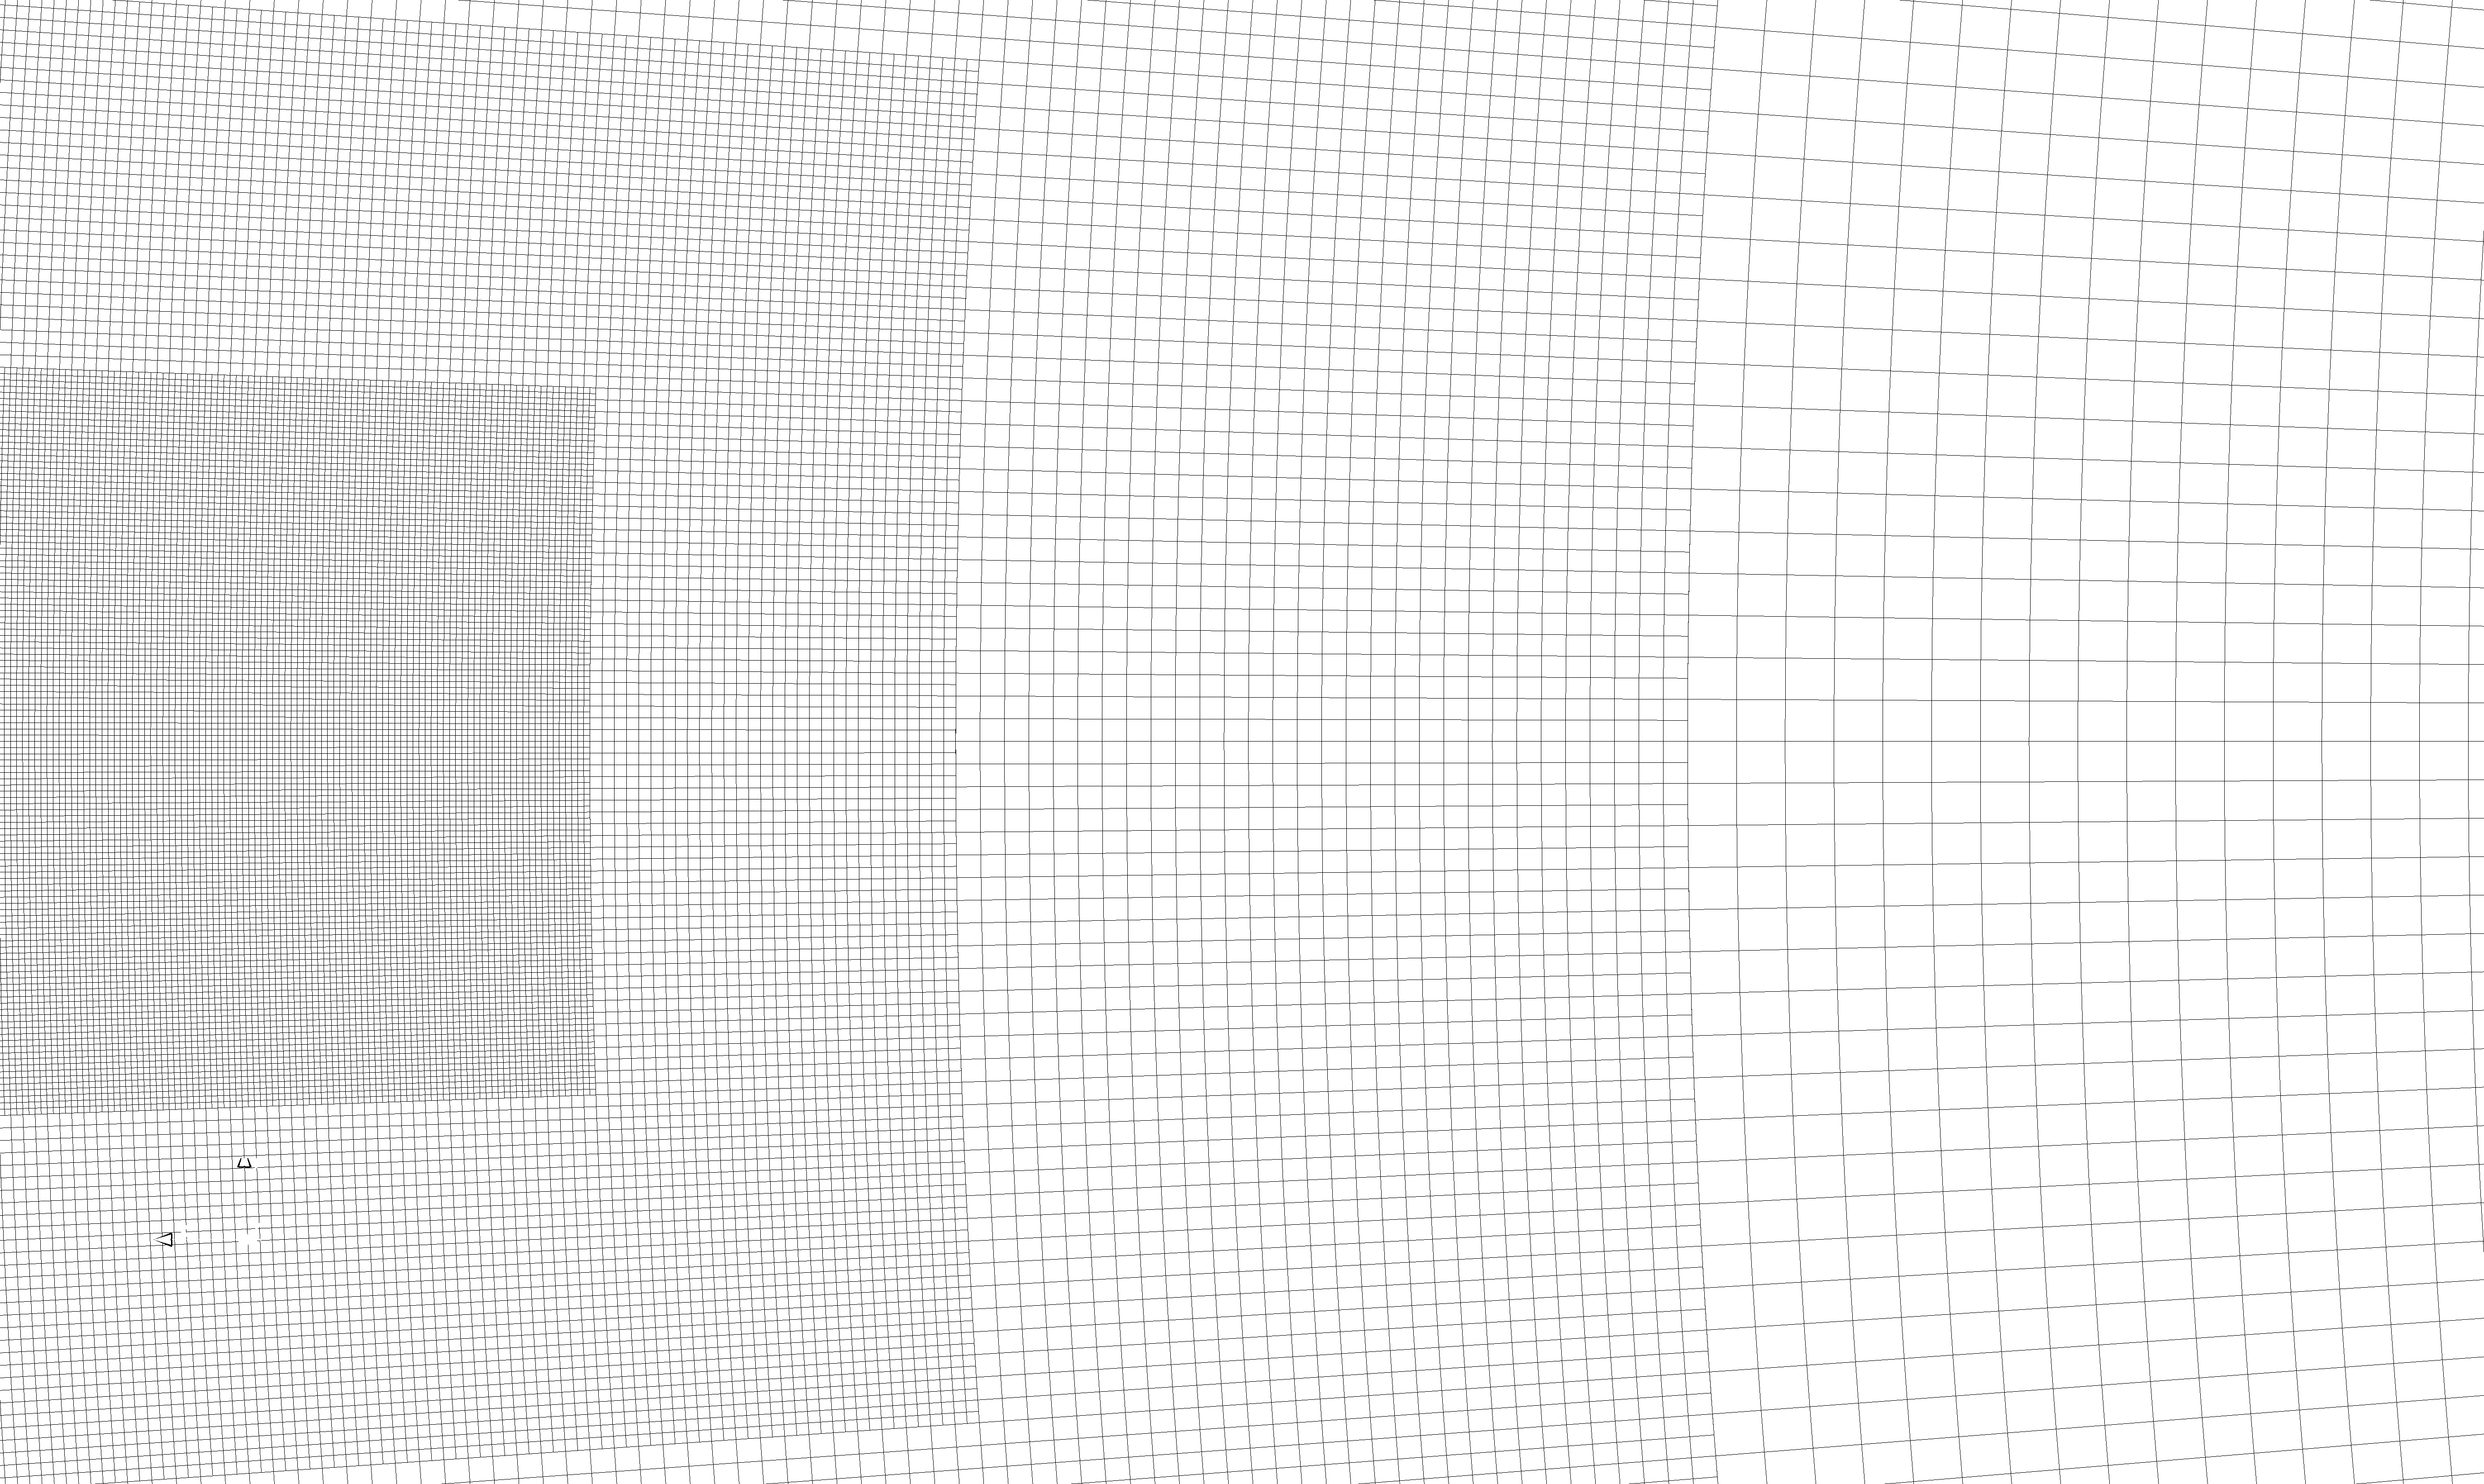
\includegraphics[width=\linewidth]{figures/Presentation/meshface.png}
	\caption{\label{fig:mesh}2D projection of nested mesh levels around the location of the planet from a JUPITER simulation.}
\end{figure}

When using adaptive or multigrid solvers, the results of computations at one refinement level are used to provide the initial conditions for the next level to reduce computation time, and is shown in Fig. \ref{fig:vcycle}. 
Starting with the finest grid, a first solution is found. 
This solution is \textit{restricted} to the overlapping region of the next finest grid. 
This process is repeated to the coarsest grid, where the full solution is calculated.
These results are then \textit{prolongated} down to the finer mesh, and again all the way back to the finest level, where a solution is achieved. 
This process can then be iterated, and is known as the v-cycle \cite{hockney1988computer}.

\begin{figure}
	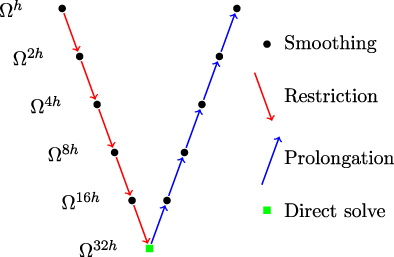
\includegraphics[width=\linewidth]{figures/Presentation/vcycle.jpg}
	\caption{\label{fig:vcycle} Example of a v-cycle for a 6 level multigrid \cite{vcycle}.}
\end{figure}

\subsection{Outputs}\label{sec:out}
As JUPITER relies on parallel computation, each computational core will output the hydrodynamic fields in its mesh region. These can be stitched together to create output files for each hydrodynamic field over the whole disk.

The first output file is a descriptor file that provides simulation properties, along with the positions in spherical coordinates of each of the vertices of the mesh for each mesh level. 
For this report $\phi$ represents the azimuthal angle, and $\theta$ the polar angle from the z-axis, and coordinates are generally ordered ($\phi$, $r$, $\theta$). 
The file is structured as follows:
\begin{lstlisting}
[line 1]
[line 2]
[line 3]
[line 4]
[line 5]
[line 6]
[N$_{\phi}$ N$_{r}$ N$_{\theta}$]
[line 8]
[$\phi$ axis]
[$r$ axis]
[$\theta$ axis]
\end{lstlisting}
This structure is then repeated sequentially for each mesh refinement level, from coarse to fine. The lines without descriptions are undocumented lines used within the JUPITER simulations, and are not relevant for this report. The first and last two components of each axis are ghost cells, and should not be read in. The number of components along each axis (e.g. $N_{\phi}$) takes this accounts for this, however it assumes zero index counting. Thus if there are $n$ $\phi$ components, the descriptor file will read $n-1$, and the total $\phi$ axis in the file will contain $n+4$ elements.

Each hydrodynamic field is stored in a data file, with a data point for each cell of the mesh. Note that while the descriptor file stores the locations of the vertices of the cells, all of the field data is defined at the barycentre of a given cell. The data is stored as binary doubles, and is ordered such that for a given coordinates ($\phi_{i}$, $r_{j}$, $\theta_{k}$), $i$ is iterated the fastest and $k$ the slowest. For vector data (velocities), each component of the vector is ordered as a scalar, with the azimuthal velocity listed first in its entirety, followed by the radial component, followed by the polar component. This ordering is also user adjustable in JUPITER, and may change. All data is stored in code units, and must be converted to physical units after read in.

Many of these hydrodynamic fields cannot be processed for visualisation with existing software (e.g. RadMC3D), so a conversion tool was necessary to allow for visualisation in Paraview.
\section{Processing Tools}\label{sec:code}
All of the tools described on this section are available on Github: \url{https://github.com/nenasedk/JUPITER_VTKFileConversion}. 
\subsection{VTK File Structure}\label{sec:vtk}
Paraview uses the VTK file format to store data for visualisation. This section describes the format as in \cite{Formats2009}. While a modern XML format exists, the legacy format is simpler to use and has much more extensive documentation, and was thus chosen for this project. Future work could explore the usage of a VTK format developed for adaptive mesh grids.

The legacy VTK format is structured into 5 parts:
\begin{enumerate}
	\item The file version and identifier, which must be exactly \verb|# vtk DataFile Version x.x|
	For this project we are using VTK version 2.0.
	\item The header, one line terminated by \verb|\n| to describe the data.
	\item File format. Either \verb|ascii|$\lvert$\verb|binary|
	\item Dataset structure. This describes the geometry and topology of the dataset, and consists of the word \verb|DATASET| followed by a keyword description of the data. We use an Unstructured Grid to describe the data.
	An unstructured grid requires both a list of coordinates and a list of connections to fully specify the locations and connections of each cell in the grid.
	
	Following the keyword is the list of coordinates used to describe the data. This initiated by line \verb|POINTS n datatype|, where n is the number of coordinates and datatype is a C type (we use doubles). The JUPITER coordinate grid is listed in order $\phi$, $r$, $\theta$, with $\phi$ iterating the fastest and $\theta$ the slowest. Each coordinate vector is converted to a Cartesian grid before being written to file, so the VTK file will contain the x,y,z components of each vertex in the mesh in CGS units, centred on the star. Each mesh level is appended subsequently from coarsest to finest. 
	
	After the list of coordinates, the cells are listed. This section begins with the line \verb|CELLS m| where m is the number of cells. Each row begins with the number of vertices of the cell, followed by the index of the coordinates of each vertex of the cell. We use a hexahedral cell type (cell type 8), and a description of the algorithm to compute the indices is found in Sec. \ref{sec:code}. Although the JUPITER grid is based in spherical coordinates, for a small enough grid size a Cartesian grid with hexahedral cells provides a `close-enough' approximation for practical purposes.
	
	Following the list of cells is the list of cell types for each cell. This is started by the line \verb|CELL_TYPES m| where m is the number of cells. All of the cells used in JUPITER are hexahedral (type 12).
	\item Dataset attributes. This can be either \verb|POINT_DATA|, where each datapoint is located at a mesh vertex, or \verb|CELL_DATA|, where each datapoint is located at the centre of a cell. All JUPITER hydro fields are \verb|CELL_DATA|. Additionally, each datapoint can be either a \verb|SCALAR| or \verb|VECTOR|, the latter of which is used to store velocities.
\end{enumerate}
An example file is included in Appendix A.
\subsection{Data Processing Methods}\label{sec:proc}
\textbf{Requirements}

To run the python conversion script the user must have installed at minimum: Python 2.7, numpy, astropy and the python VTK package v8.1.1. 
It is recommended to use the environment included with the package on Github.

\textbf{Overview}

To process the outputs of the JUPITER simulations into the VTK file format, a python class was written. 
The class has a range of user settable functions, allowing the user to write a script to wrap the class for a given conversion job, or use the interactive command line interface written for the class.
In general, the user must provide the input and output directories, the output number, the number of mesh refinement levels, the hydrodynamic field to convert, the orbital radius of the planet in AU and the mass of the star in solar masses.

The other primary requirement of the tool was to be at most of O(n) time complexity, as the mesh can contain millions of elements. This restricts which algorithms can be used throughout the program.

The program flow is as follows:
\begin{enumerate}
	\item Set-up directories and filenames, and set science variables.
	\item Read in the coordinates from the descriptor file. From the axes read in, build a grid of 3D coordinates ($\phi_{i}$, $r_{j}$, $\theta_{k}$), and create an additional grid with the coordinates converted to Cartesian. 
	\item For each mesh level, define the boundaries of the next finest level. Cells (NOT grid points) within this region of interest (ROI) will be ignored.
	\item Compute the indices of each vertex of each cell. This is achieved using a stride calculation in the \verb|ComputeStructuredCell()| function:	
	\begin{itemize}
		 \item Label the indices from 0 to 7, counter clockwise and from bottom to top as shown in Fig. \ref{fig:cube}.
		 \item The $\phi$ axis is iterated fastest and $\theta$ the slowest. Therefore index 1 will be one greater, but index 3 will be a full $\phi$ axis farther along than index 0. Likewise, index 4 will be an $r-\phi$ plane greater than index 0.
		 \item Iterate through each axis, incrementing the counters. Any cells with one or more vertices within the ROI will be skipped, but their index in the total list of cells is stored.
 	\end{itemize}
	\item Read in the data from the descriptor file, reshaping vector (velocity) data as necessary. Remove the datapoints with the indices of the removed cells.
	\item Write the data to a binary or ascii VTK file. If the output file already exists, the user can choose to overwrite the file, or append new data to the existing file.
\end{enumerate}
\begin{figure}[t]
	\centering
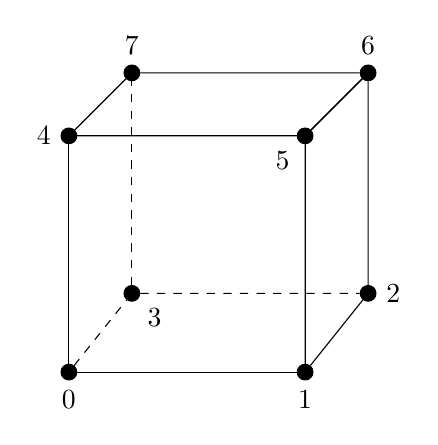
\begin{tikzpicture}
\foreach \n/\x/\l/\p in{
	1/{( 0  , 0)}/{$0$}/below,
	2/{( 3, 0)}/{$1$}/below,
	3/{( .8, 1)}/{$3$}/south east,
	4/{( 3.8, 1)}/{$2$}/right,
	5/{( 0, 3)}/{$4$}/left,
	6/{( 3, 3)}/{$5$}/south west,
	7/{( 0.8, 3.8)}/{$7$}/above,
	8/{( 3.8, 3.8)}/{$6$}/above
}
{
	\node[inner sep=2pt,circle,draw,fill,label={\p:\l}] (\n) at \x {};
}
\draw (1) -- (2) -- (6) -- (5) -- (1);
\draw (5) -- (6) -- (8) -- (7) -- (5);
\draw (2) -- (4) -- (8) -- (6) -- (2);
\draw[dashed] (1) -- (3) -- (4);
\draw[dashed] (3) -- (7);
\end{tikzpicture}
\caption{\label{fig:cube} Labelling of hexahedral cell vertices. 0-1 lies along the azimuthal axis, 0-3 along the radial and 0-4 along the polar axis. Each vertex is labelled using the ordering of the grid read in from file, that is the index of vertex 3 is an length(azimuthal axis) greater than vertex 0, where the length of the axis is the number of points in the axis. Likewise, vertex 4 iterates over both the azimuthal and radial axes, so its index is length(azimuthal axis)$\times$length(radial axis) greater than vertex 0.}
\end{figure}
\textbf{Usage}

To use the command line interface simply use \verb|python Convert.py|.
Within the Convert.py script, the user can change whether to output to a binary or ascii VTK file, as well as the location of the input data from JUPITER. This data must be in a folder labelled outputXXXXX where the X's denote the simulation output number with leading zeros. The default path to this directory is the current working directory.

A second interface has been developed to allow for easier bash scripting. To use this, enter the following into the command line or a bash script:
\verb|python script_Convert.py [first]\|\newline \verb|[grid level] [radius] [mass]|\newline \verb|[-l [last]] [-v]\| \newline \verb|[-b [binary/ascii]] [-d[dir]]\ |\newline\verb|[-f [field list]]|

Or without all of the optional tagged arguments:\newline
\verb|python script_Convert.py [first]\|\newline \verb|[grid_level] [radius] [mass]\|\newline \verb|[-f [field list]]|

Tagged arguments can be placed in any order, but the field list must be the last argument passed.
\begin{itemize}
	\item \verb|[first]| The first simulation output to process.
	\item \verb|[-l [last]]| The last simulation output to process. Assumes that all integers between first and last exist and should be processed.
	\item \verb|[grid_level]| The mesh refinement level.
	\item \verb|[radius]| The orbital radius of the planet in AU.
	\item \verb|[mass]| The mass of the star in solar masses.
	\item \verb|[-v]| Include if velocities should be planet centred. 
	\item \verb|[-b [binary/ascii]]| A string (b)inary or (a)scii to set the output file type. Binary is recommended, and is the default value.
	\item \verb|[-d [dir]]| Directory where the output folder from JUPITER is located
	\item \verb|[-f [field_list]]| A list of space separated strings denoting which hydro fields should be converted.
\end{itemize}
\subsection{Technical Challenges}
Several technical challenges needed to be overcome to implement this data processing tool.
\paragraph{Cell Counting}
To visualise data in Paraview, cells cannot overlap, but the output from JUPITER contains overlapping cells within the ROI around the planet. 
This creates challenges when indexing the vertices of cells, as the axis length is not constant.
However, Paraview does allow grid points to occur without being used. 
This allows us to store the full set of mesh points in the VTK file, and use a standard stride method with constant length axes to index cell vertices.
Any cells with a vertex within the ROI are discarded, with the cell number being noted to allow for removal of the datapoint.

\paragraph{Velocity Vectors}
The conversion of the velocity vectors from the initial data file to the VTK file was not straightforward. 
In the initial data file, the velocity vectors are stored component-wise, with the full list of azimuthal velocity components, followed by the radial and finally the polar velocities.
These velocities have the azimuthal velocity of the planet subtracted, so we are in the co-rotating frame of the planet.
These velocities are then converted from spherical to Cartesian coordinates using the following set of transformations:
\begin{align}
\begin{split}
&\dot{x} =\ \dot{r}\sin{\phi}\sin{\theta} +\\&\qquad\: r\dot{\phi}\cos{\phi}\sin{\theta} +\\&\qquad\: r\dot{\theta}\sin{\phi}\cos{\theta}
\end{split}\\
\begin{split}
&\dot{y} =\ -\dot{r}\cos{\phi}\sin{\theta} +\\&\qquad\: r\dot{\phi}\sin{\phi}\sin{\theta} -\\&\qquad\: r\dot{\theta}\cos{\phi}\cos{\theta}
\end{split}\\
&\dot{z} =\ \dot{r}\cos{\theta} - r\dot{\theta}\sin{\theta}
\end{align}
Where a dot denotes the time derivative of the coordinate.
Note that the direction of the y component is inverted from the standard transformation.
\section{Visualisation}
\subsection{Paraview}
\begin{figure}
	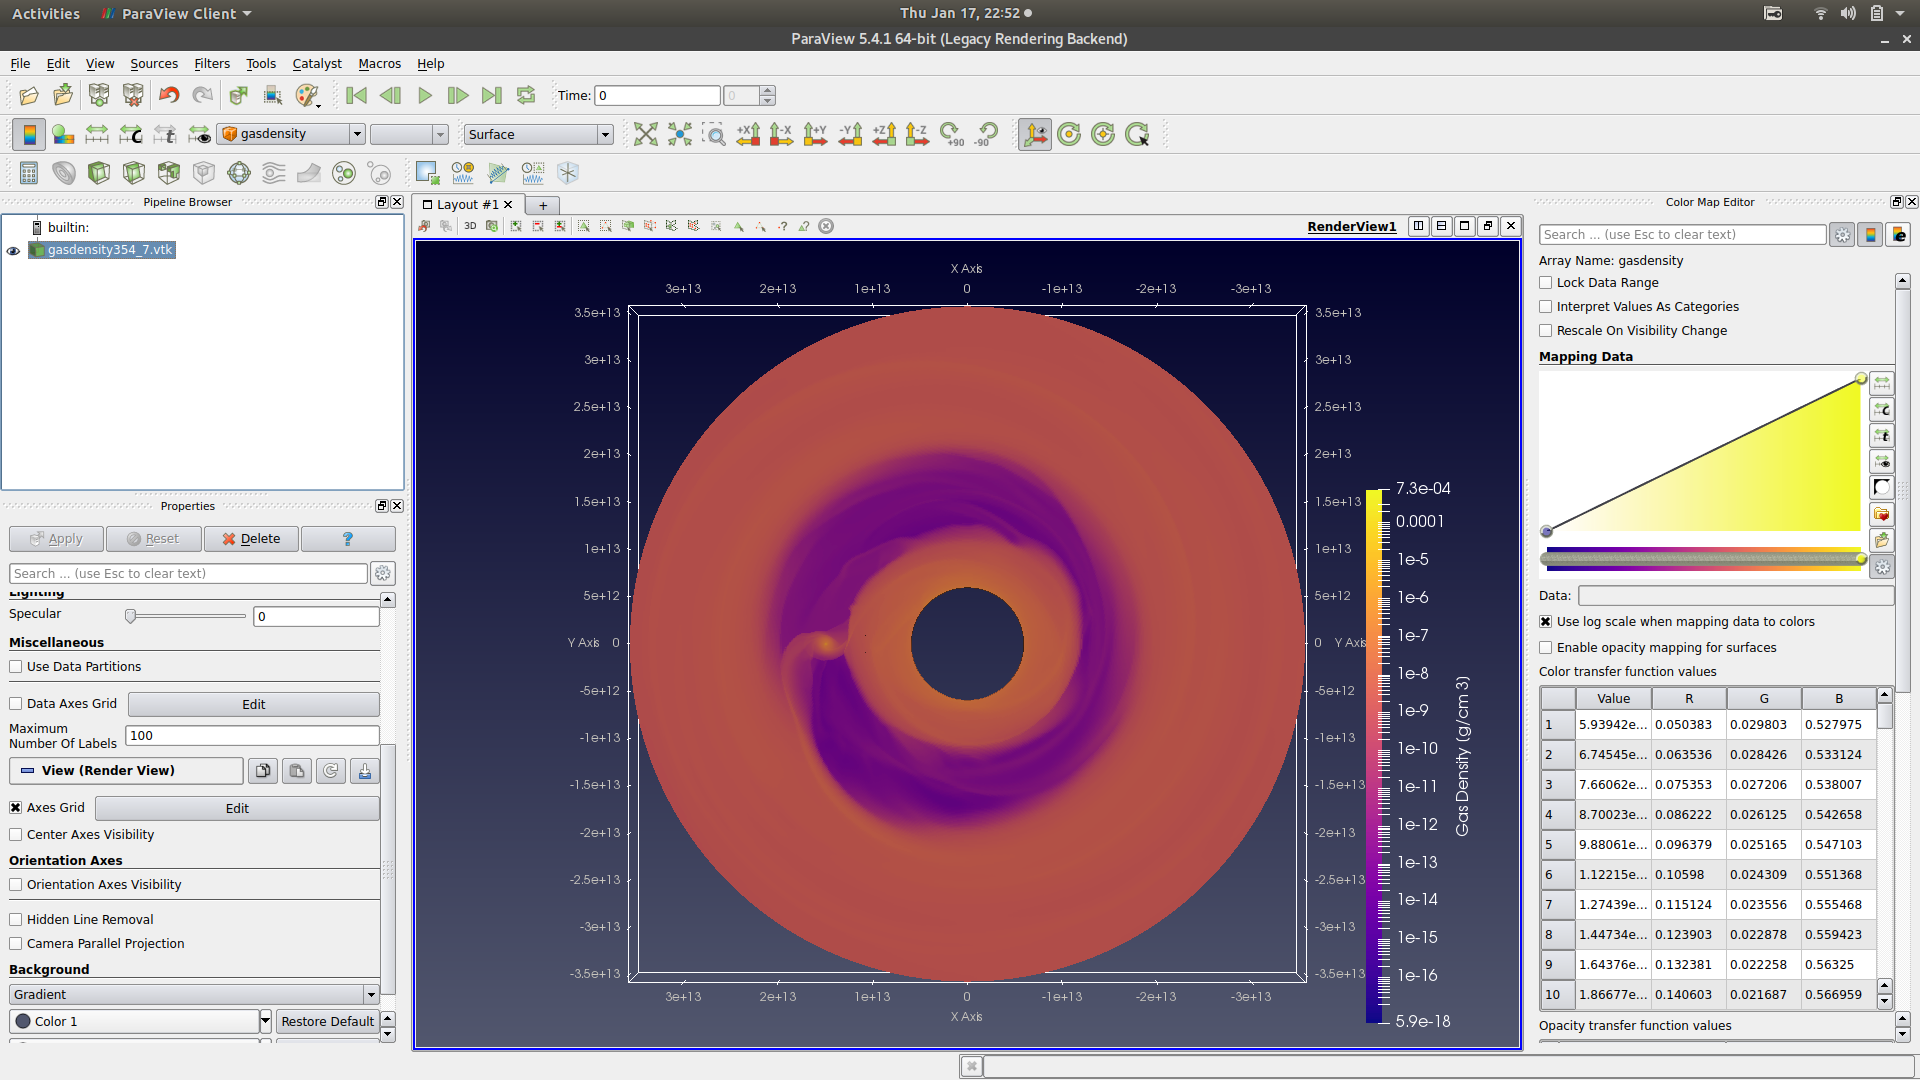
\includegraphics[width=\linewidth]{figures/Presentation/paraview.png}
	\caption{\label{fig:pviewinter}The Paraview 5.4.1 graphical user interface on an Ubuntu system.}
\end{figure}
Paraview is an interactive visualisation program that allows the user to visualise large datasets,with the processing done either in serial on a local machine or distributed on a server.
As with the VTK file format, Paraview is an open source project primarily developed by Kitware, with additional funding and support from the Sandia and Los Alamos National Laboratories.
While the full scope of Paraview's visualisation tools is extensive, and detailed in the user guide \cite{para}, we will outline some of the common techniques relevant to this report.

The render view of the Paraview user interface is shown in Fig. \ref{fig:pviewinter}.
Once a VTK file has been produced by the conversion tool, it can be opened in Paraview, where he user may then select a suitable colour map for the data. 
Best practices should be followed when producing publication-ready visualisations. Colour hue and brightness should be considered to allow for accessible images that can convey the content of the data. A large range in brightness and hue will allow small variations in the data to be more visible. 
The luminosity should be consistent across the colour range, so as not to emphasise certain features and to maintain even perception of colour intensity. 
Many pre-made colour palettes are available in Paraview, including standard matplotlib palettes commonly used in python or Matlab visualisations, allowing for standardisation across various tools.
Opacity scaling, and logarithmic colour scales are also useful tools when visualising complex data.

\begin{figure}
	\centering
	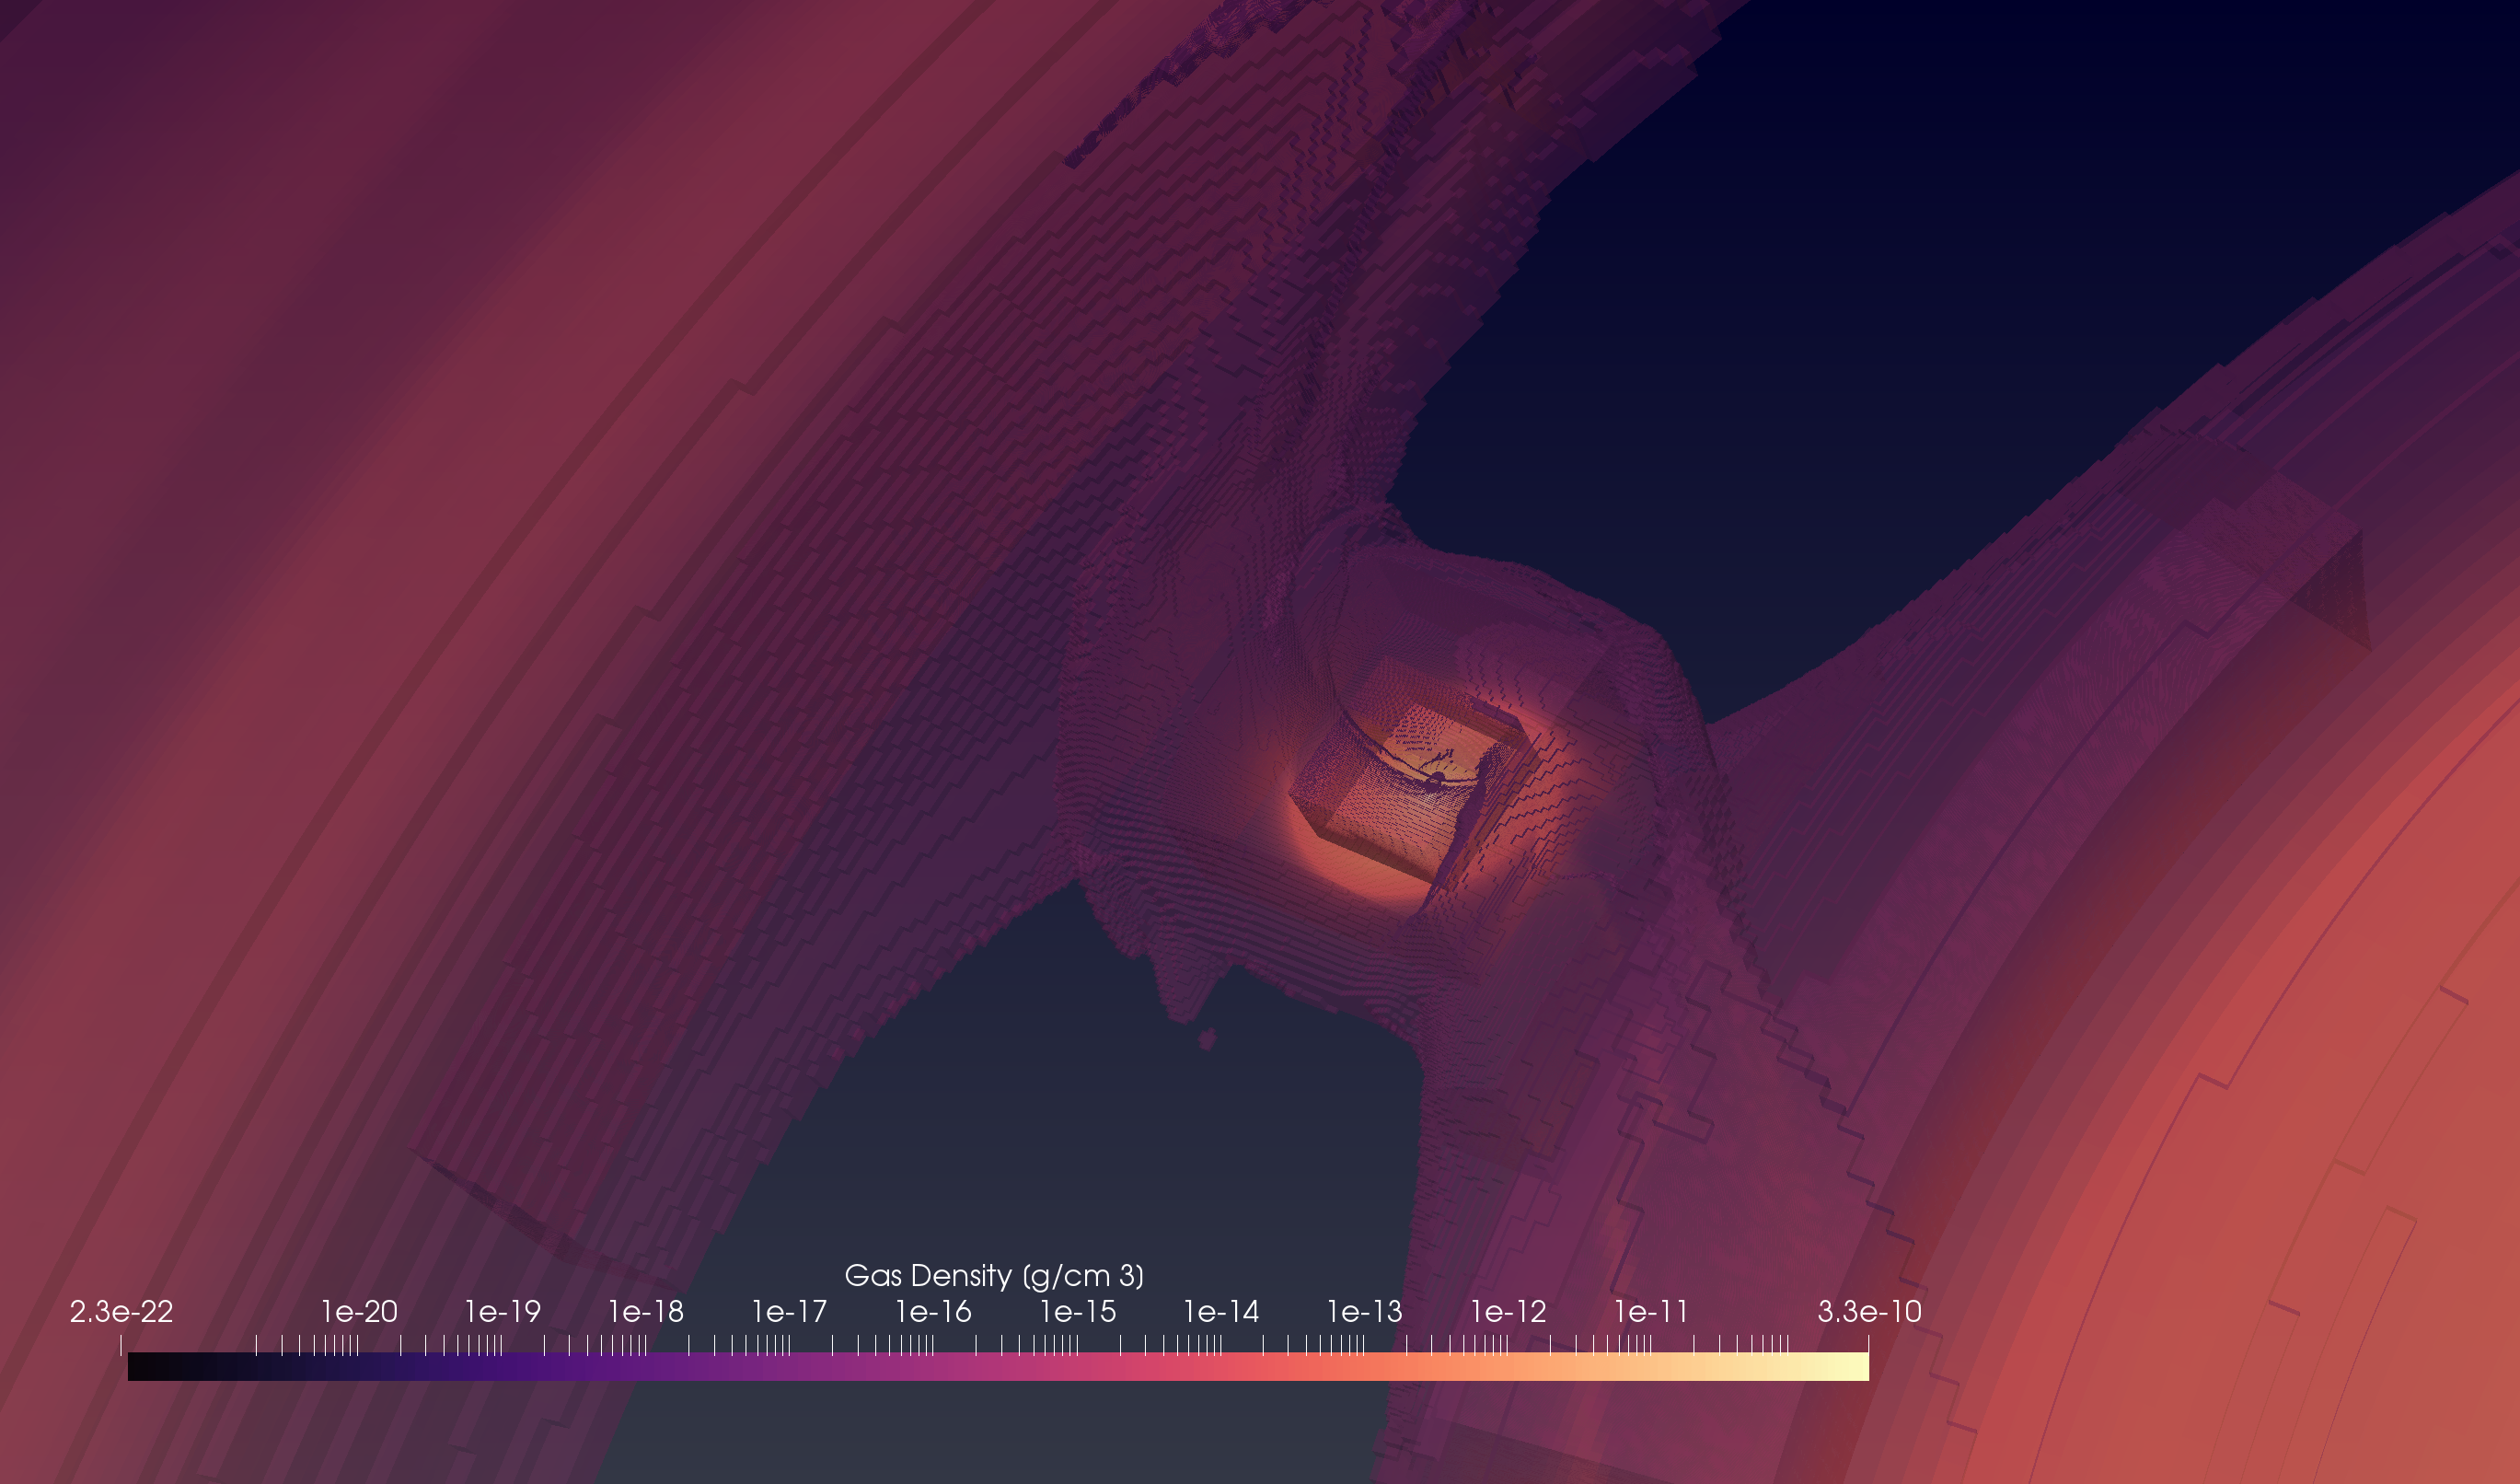
\includegraphics[width=\linewidth]{figures/DensityStructure3D.png}
	\caption{\label{fig:d3d} Example of the 3D density structure of the circumplanetary disk as rendered in Paraview.}
\end{figure}

In addition to colour, Paraview also allows the user to select various ways of representing the data in a 3D render. The default is to view the surface of the object, additional options can represent the data as points in space, a volume render, a wireframe or other options. These can be used to develop a better understanding of the 3 dimensional nature of the data, as shown in Fig. \ref{fig:d3d}.

Following the initial rendering, \textbf{filters} can be applied to the data.
Paraview currently includes around 120 different filters, several commonly used ones are summarised here.

\begin{itemize}
\item[]\textbf{Slice}
Extract a 2D slice from 3D data given an orientation and position.

\item[]\textbf{Reflect}
Mirrors the data across a specified axis.

\item[]\textbf{Clip}
Given an orientation and position, remove all cells `outside' of the cut. To generate publication quality plots, the data should be clipped down to the region of interest, as the axes will only be generated over the extent of the data.

\item[]\textbf{Threshold}
Remove all cells below a minimum, or above a maximum threshold.

\item[]\textbf{Glyphs}
Visualise vector data as arrows or other objects for flow visualisation. Typically set to show every nth vector.

\item[]\textbf{CellDataToPointData}
This filter shifts data from being located at the centre of cells to the vertices of the cell. This is required for plotting surface vectors or converting to numpy arrays.

\item[]\textbf{Surface Vectors}
This filter projects a three dimensional vector field onto a 2D plane.

\item[]\textbf{Stream Tracer}
Compute particle trajectories in a flow and visualise using streamlines. The user should set an initial point, with a small radius, and select whether to integrate forwards or backwards from that point (or both). For speed, an RK2 integrator is suggested. Typically only a small number of streamlines are necessary to visualise the flow. Used in conjunction with slicing and surface vectors, the stream trace filter can generate 2D streamline plots.

\item[]\textbf{Tube}
Replace the streamlines generated by a Stream Tracer filter with 3 dimensional tubes, for easier viewing.

\item[]\textbf{PlotOverLine}
Plots a scalar data variable along a path, such as the density along a radial line.
\end{itemize}
All of these filters can be combined in various ways to generate interesting and informative visualisations. Velocity vectors can be plotted over density fields; multiple slices can show the 3D structure of the temperature field. Additional tools include axis visibility, with customisable labelling, background settings (solid colour, gradient or image), alternate render views (slice view, charts, etc.) animations and more.

\subsection{Paraview Processing Example}
A typical example of a desired output would be a publication ready, 2D plot of a velocity vector stream on top of a scalar field such as the temperature. 
To produce this plot, read in both the temperature and velocity VTK data files. 
Slice the data along the desired axis to produce a 2D surface plot, and clip the data to the region of interest. 
Filter parameters can be copied and pasted, so identical filters can be applied to both datasets.
Choose a colourmap and scale for the temperature field, and label the colourbar axis. 
Ensure the axis are visible, properly labelled and with a reasonable font size chosen.
Apply the CellDataToPointData filter to the sliced and clipped velocity data, followed by the surface vector filter.
Finally, generate a stream plot, and colour the streams with the magnitude of the velocity.
Ensure the render background is white, and position the colourbars where desired. Save the scene in the desired file format, or export as a png screenshot. 
Note that both of these output options may not exactly reproduce the render view, so check the final output to ensure consistency.
The output of this procedure should resemble Fig. \ref{fig:tshock}.%\ref{FIXME}.

\subsection{VTK Python}\label{sec:pyvtk}
An alternative to Paraview that allows for automation of plot generation is the python wrapper for the C++ based VTK library \cite{avila2010vtk}.
The python VTK package maintains the same functionality as Paraview, and produces similar results as it uses the same rendering engine.
Fig. \ref{fig:vtkpipe} outlines the process of generating a render using the VTK package.
A VTK file is read in with a \verb|reader| module. Each variation of the VTK grid structure (rectilinear, unstructured, XML, etc.) has its own reader, so the reader must match the VTK filetype being read in. 
\begin{figure}
	\centering
	\begin{tikzpicture}[node distance = 1.3cm, auto]
	% Place nodes
	\node [block] (init) {Reader};
	\node [block, below of=init] (identify) {Filter(s)};
	\node [block, below of=identify] (evaluate) {Mapper};
	\node [block, below of=evaluate] (decide) {Actor};
	\node [block, below of=decide] (stop) {Renderer};
	% Draw edges
	\path [line] (init) -- (identify);
	\path [line] (identify) -- (evaluate);
	\path [line] (evaluate) -- (decide);
	\path [line] (decide) -- (stop);
	\end{tikzpicture}
	\caption{\label{fig:vtkpipe} The pipeline for processing VTK data in python.}
\end{figure}
The reader provides access to all of the data stored in the VTK file such as scalar or vector fields, along with the coordinate grid. 
It also details many of the properties of the file and the data stored within, including the number of points, the names and lengths of each data field, header information and more.

The data from the reader is typically accessed with the \verb|reader.GetOutput()| function, which can be passed to filter objects for processing. 
Note that some filters use the function \verb|reader.GetOutputPort()| instead.
All of the filters available in Paraview are available in the VTK package. 
It is also possible for the user to write their own filter classes, though that is beyond the scope of this report.

After the data has been passed from the reader to the filter, it is applied using a Mapper object. 
This class maps the data to graphics primitives to allow for rendering. Any object to be rendered must be passed through a mapper class.
The Mapper object is then passed to an Actor, which specifies the geometry and properties for the render. 
All Actors are then passed to the Renderer, which outputs a visualisation of the data. At each level of this pipeline, various settings are available with class functions to adjust the output of the render, for example changing the colourmap or camera position. The full documentation is available in \cite{avila2010vtk}.

The use of the VTK package was explored as a means to reliably produce publication ready plots, and allow for some level of automation and reproducibility to increase the speed of generating plots.
However, scripts must be tailored for specific datasets, reducing the utility of templates, and the lack of a visual reference leads to difficulties in producing the desired results. 
It was found that the GUI of Paraview provided a faster workflow and easier methods for generating high quality renders.

As a third alternative, the use of numpy and matplotlib was explored, as plots generated with these tools are effectively the standard in the scientific community. 
The use of these tools also relies upon the VTK python library, and an understanding of the VTK pipeline remains a necessity.

\subsection{Plotting with Matplotlib}
As matplotlib style plots are relatively standard, we developed a python program to take in the VTK files and output matplotlib plots.
The data is read in and processed as described in \S \ref{sec:pyvtk} above. 
The data must be sliced and cut using the VTK filters prior to conversion.
Once filtered and passed to a \verb|CellDataToPointData| mapper, the mapper output can be converted to numpy arrays using the \verb|vtk_to_numpy| function.
The point coordinate grid can likewise be converted to a numpy array, and read into Cartesian axes. 

\begin{figure}
	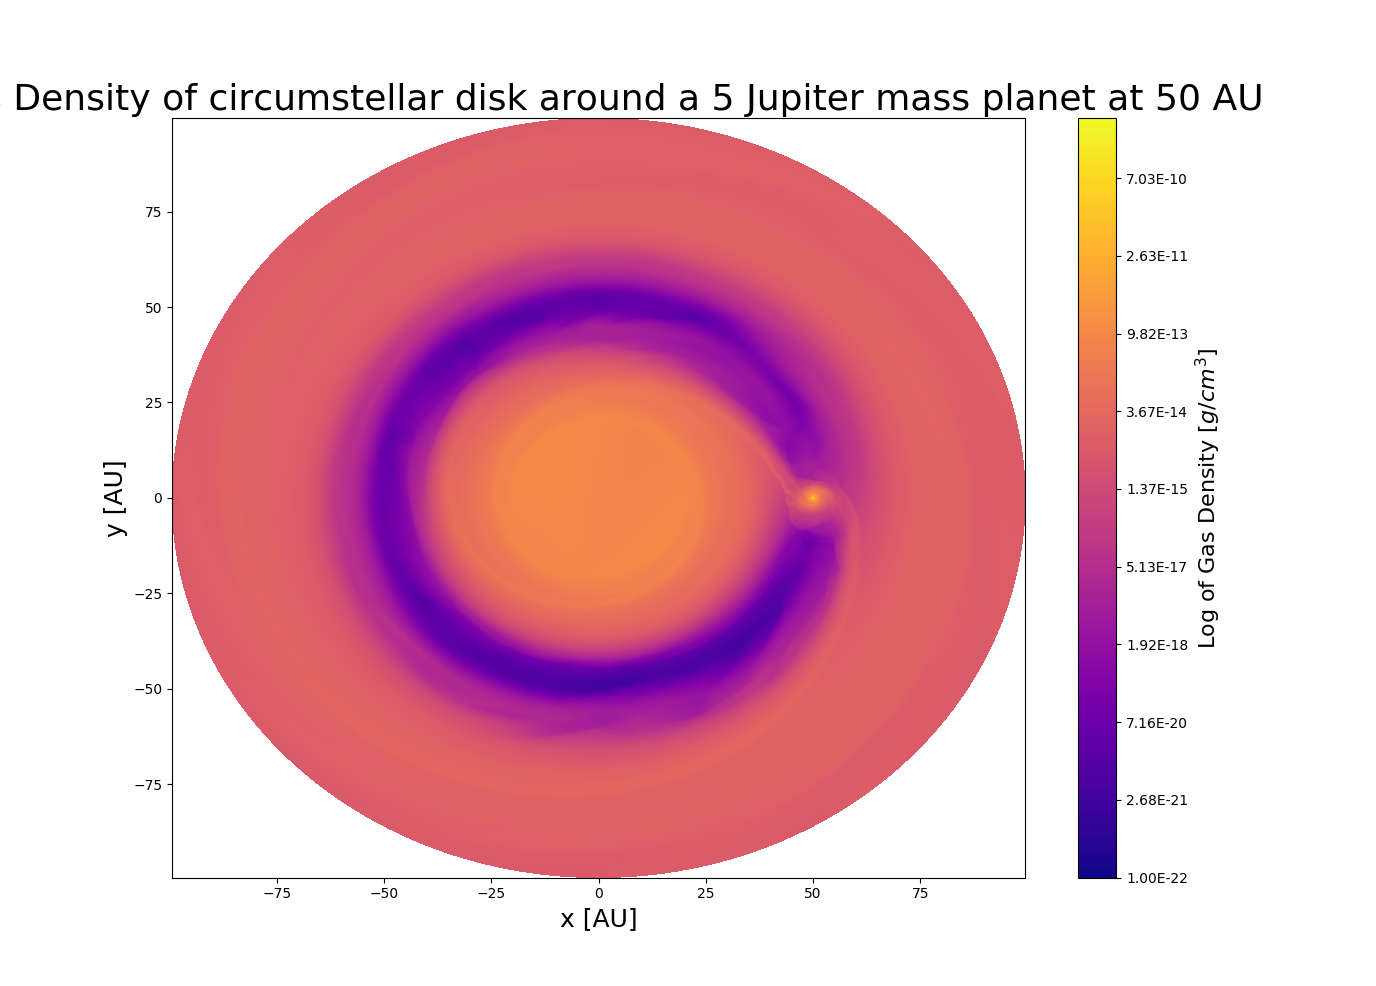
\includegraphics[width=\linewidth]{figures/Presentation/mpl.png}
	\caption{\label{fig:mpl}Matplotlib style figure of the density of a circumstellar disk.}
\end{figure}  

\begin{figure*}[htb!]
	\centering
	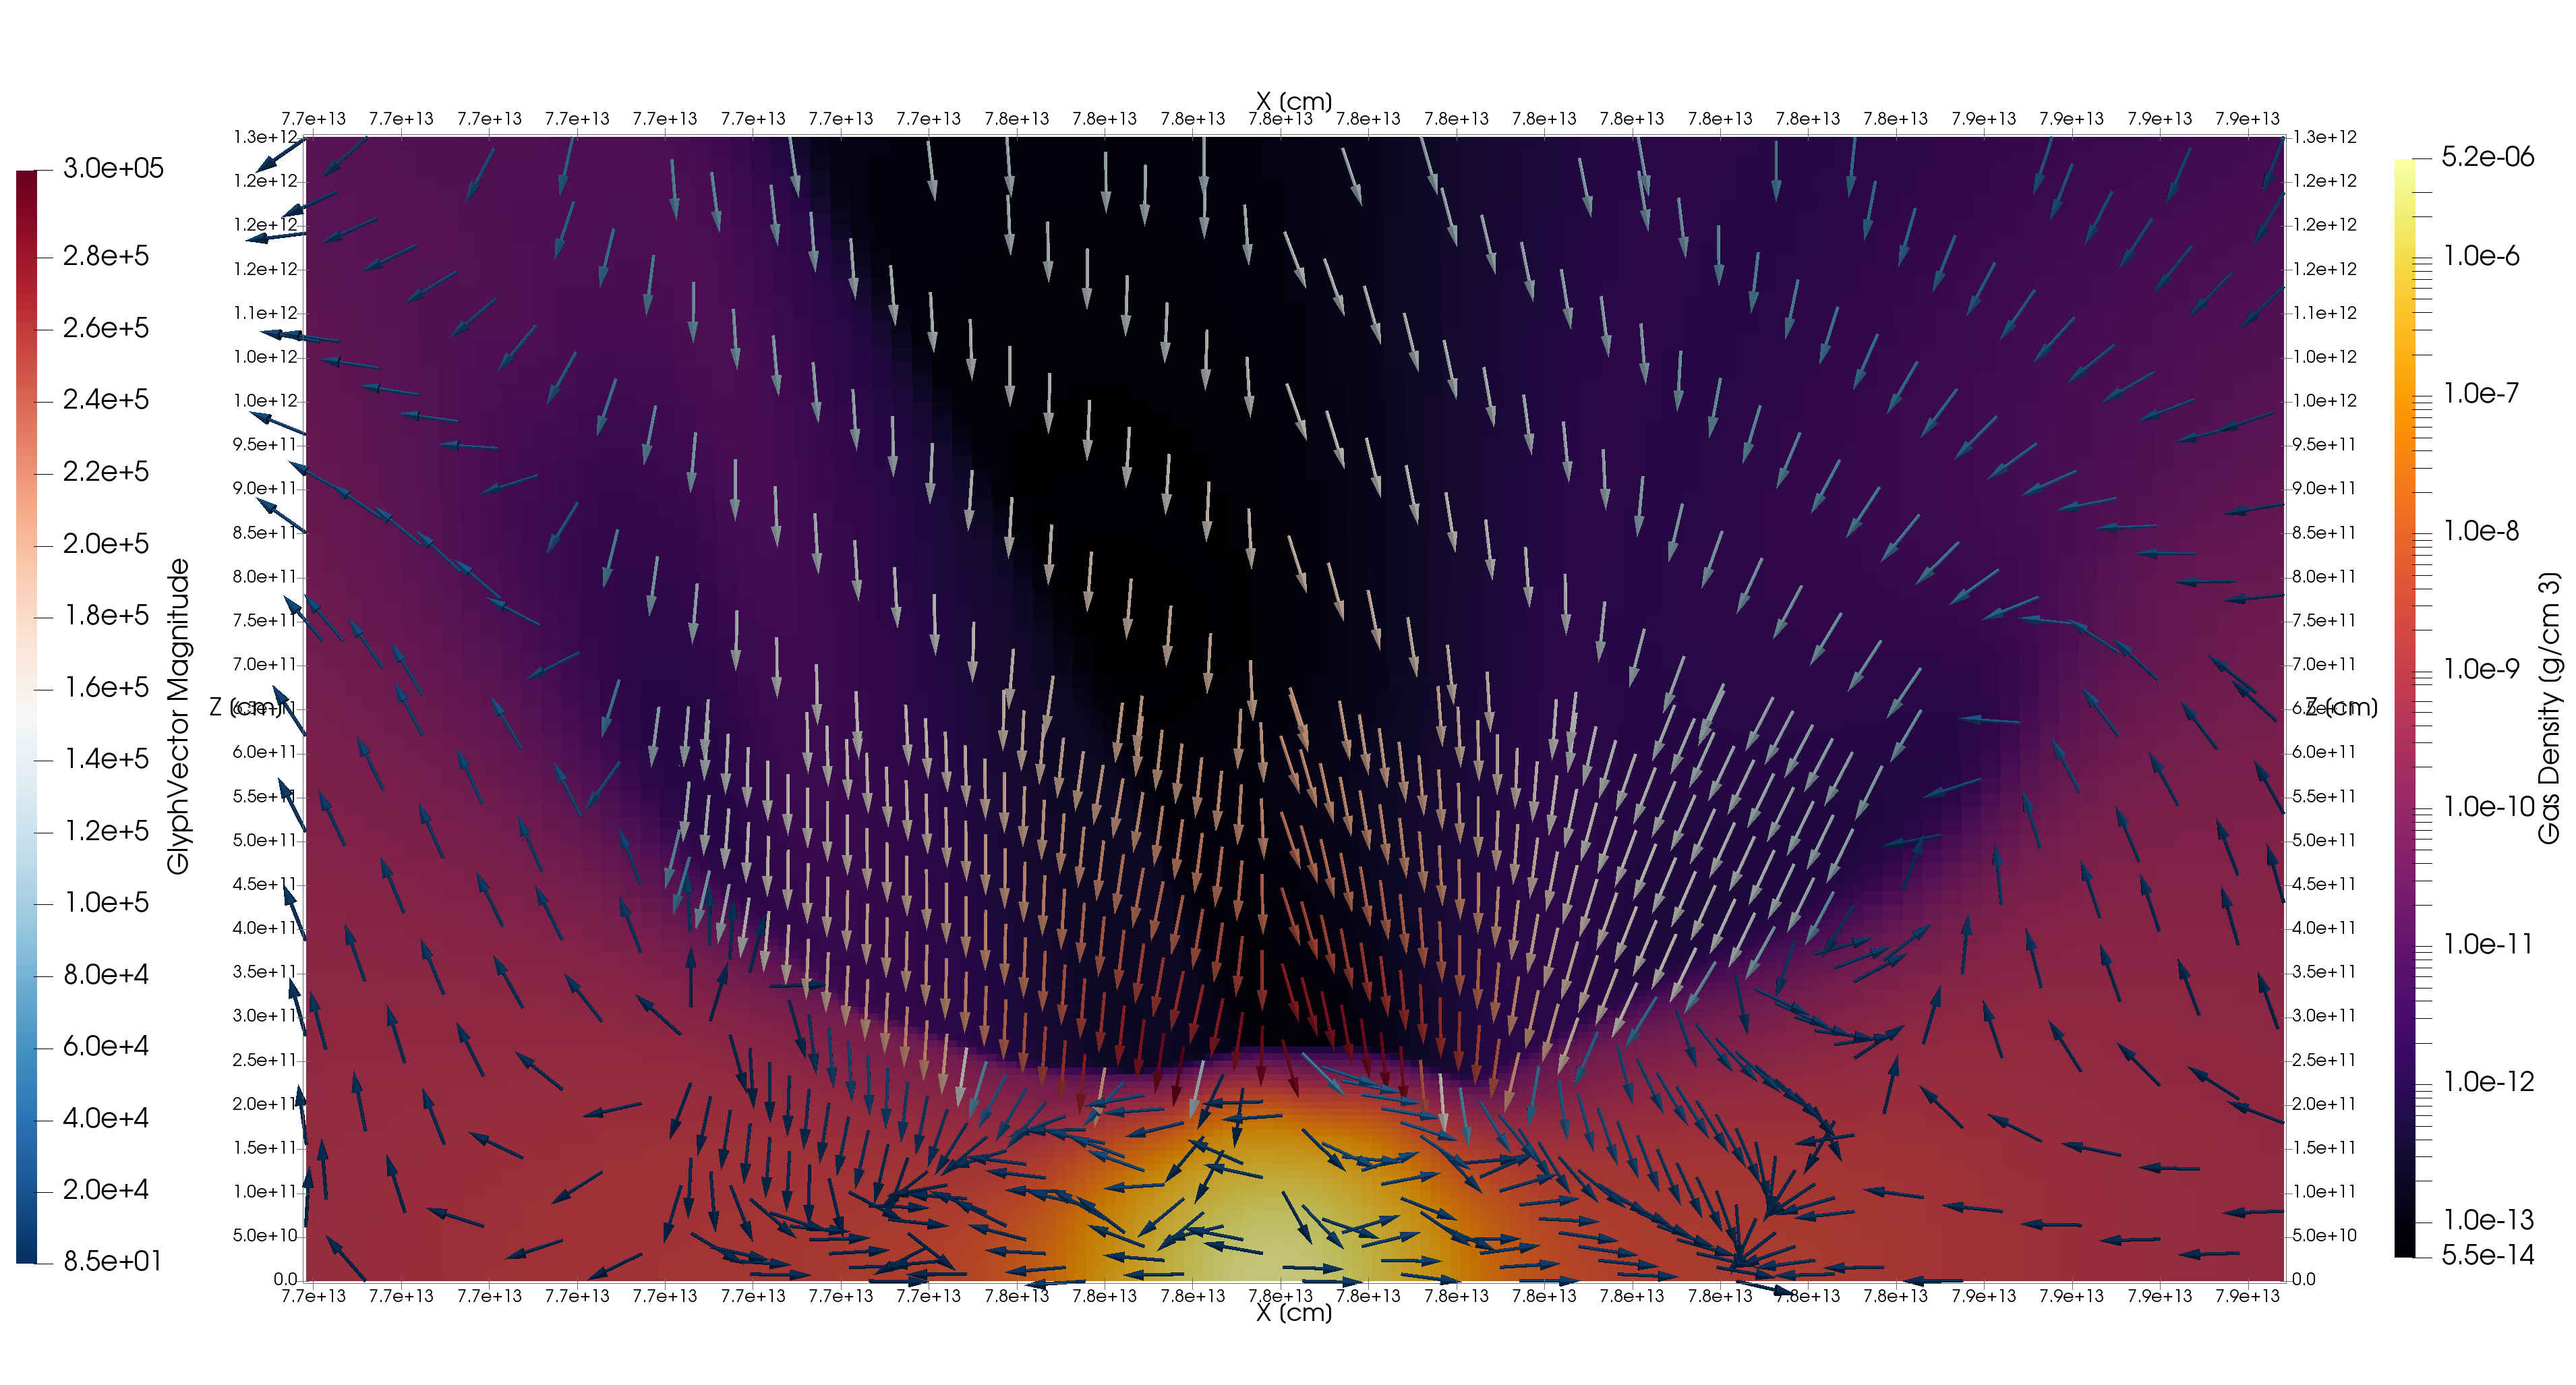
\includegraphics[width=1.0\linewidth]{figures/Presentation/OutFlowCross.png}
	\caption{\label{fig:vel} Vertical inflow of gas shocking near the surface of the accreting 1 M$_{J}$ planet, followed by the outflow of gas in the circumplanetary disk.}
\end{figure*}

We found that the function \verb|tricontourf()| produces the best outputs for scalar fields, as many other plotting functions require 2D pixel grids for each axis. 
With millions of coordinate points and an irregular grid, this quickly grows larger than the available memory on a consumer-grade computer.
\verb|Tricontourf| uses Delauney triangulation to create a grid from 1D coordinate axes, which can be irregular. The data is then mapped over the grid, and plotted with a filled contour. The resolution of the colourscale can also be specified. 
An example of the matplotlib output can be seen in Fig. \ref{fig:mpl}.

However, this style of plotting also has its limitation. 
Vector plots are difficult, and do not produce insightful results.
Stream plots are currently impossible due to the above mentioned memory issues - this is a known issue with the matplotlib Streamplot function.
Therefore, while useful for generating simple plots in a standardised format, matplotlib remains less useful for more complex visualisations.


\subsection{Results}\label{sec:res}
With the conversion tool developed, we can present several examples of possible visualisations made using Paraview \cite{para}. In this section we discuss the scientific results of a set of JUPITER simulations. 


These simulations primarily consist of 100AU radius circumstellar disks with a single embedded planet of varying mass at 50AU.
The gas in the simulations is considered to be ideal, with an equation of state and adiabatic coefficient as in Eqn. \ref{eqn:eos}
The kinematic viscosity of the simulations is low, with a value of $10^{-5}a^{2}\Omega_{p}$, or $\alpha \approx 0.004$ at R$_{p}$. The density is close to that of a Minimum Mass Solar Nebula \cite{MSMN}. 
The initial disk aspect ratio was set to H/r = 0.05, where H is the pressure scale-height of the disk. 
The upper surface of the disk is radiatively heated from stellar flux.
For the opacity calculation, the dust-to-gas ratio of the disk was set to the standard value for the interstellar medium of 0.01.

\begin{figure}[h]
	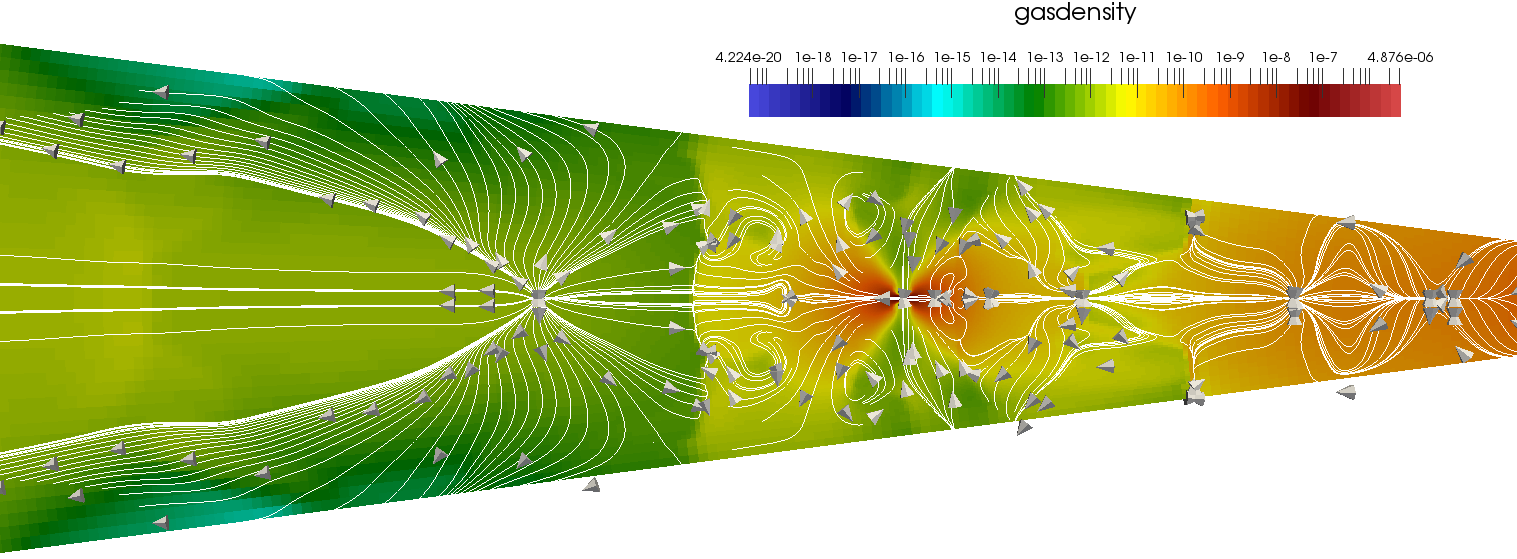
\includegraphics[width=\linewidth]{figures/Presentation/recirc.png}
	\caption{\label{fig:recirc}Meridional recirculation of gas from the CPD back into the circumstellar disk.}
\end{figure}

\begin{figure}[htb!]
	\centering
	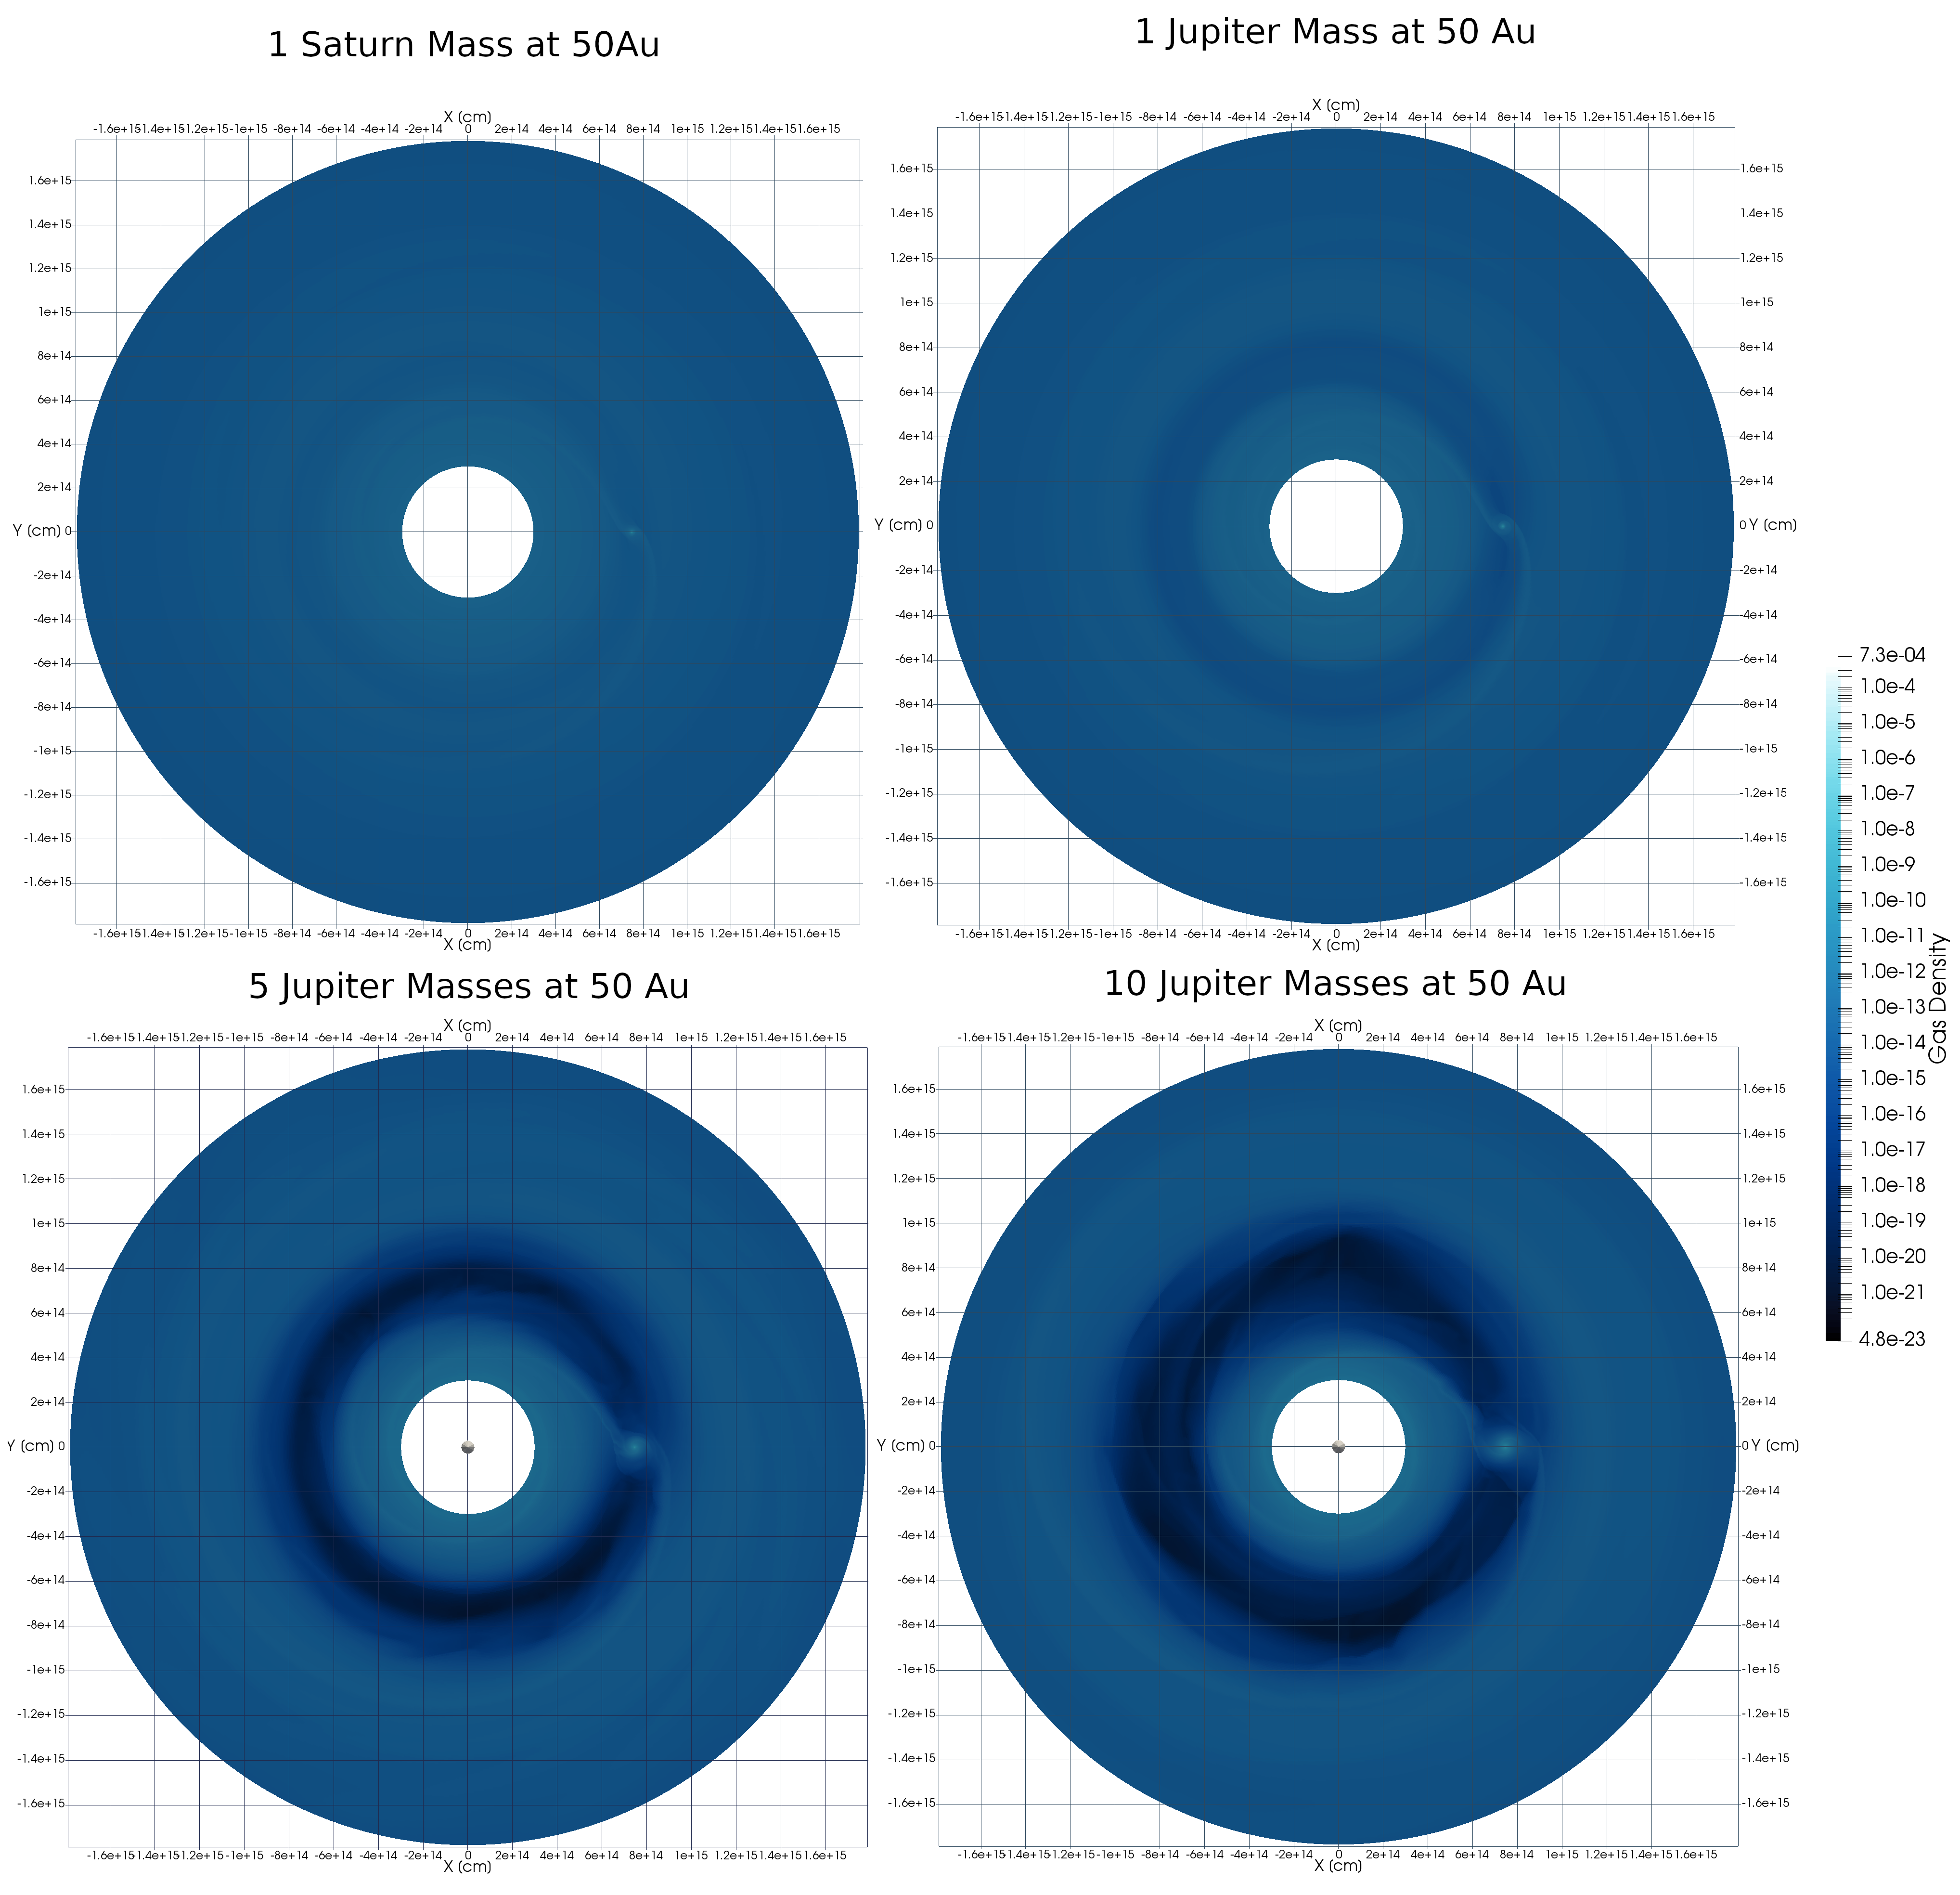
\includegraphics[width=\linewidth]{figures/Presentation/Gaps/Gaps.png}
	\caption{\label{fig:gaps}Variation of gap widths and depths over a range of embedded planetary masses. The colour scale is in units of g cm$^{-3}$. From 1 M$_{J}$ to 10 M$_{J}$, the gap width increases by a factor of 2, while the depth decreases from 8$\times10^{-16}$g cm$^{-3}$ to 5$\times10^{-20}$g cm$^{-3}$.}
\end{figure}

\begin{figure}[htb!]
	\centering
	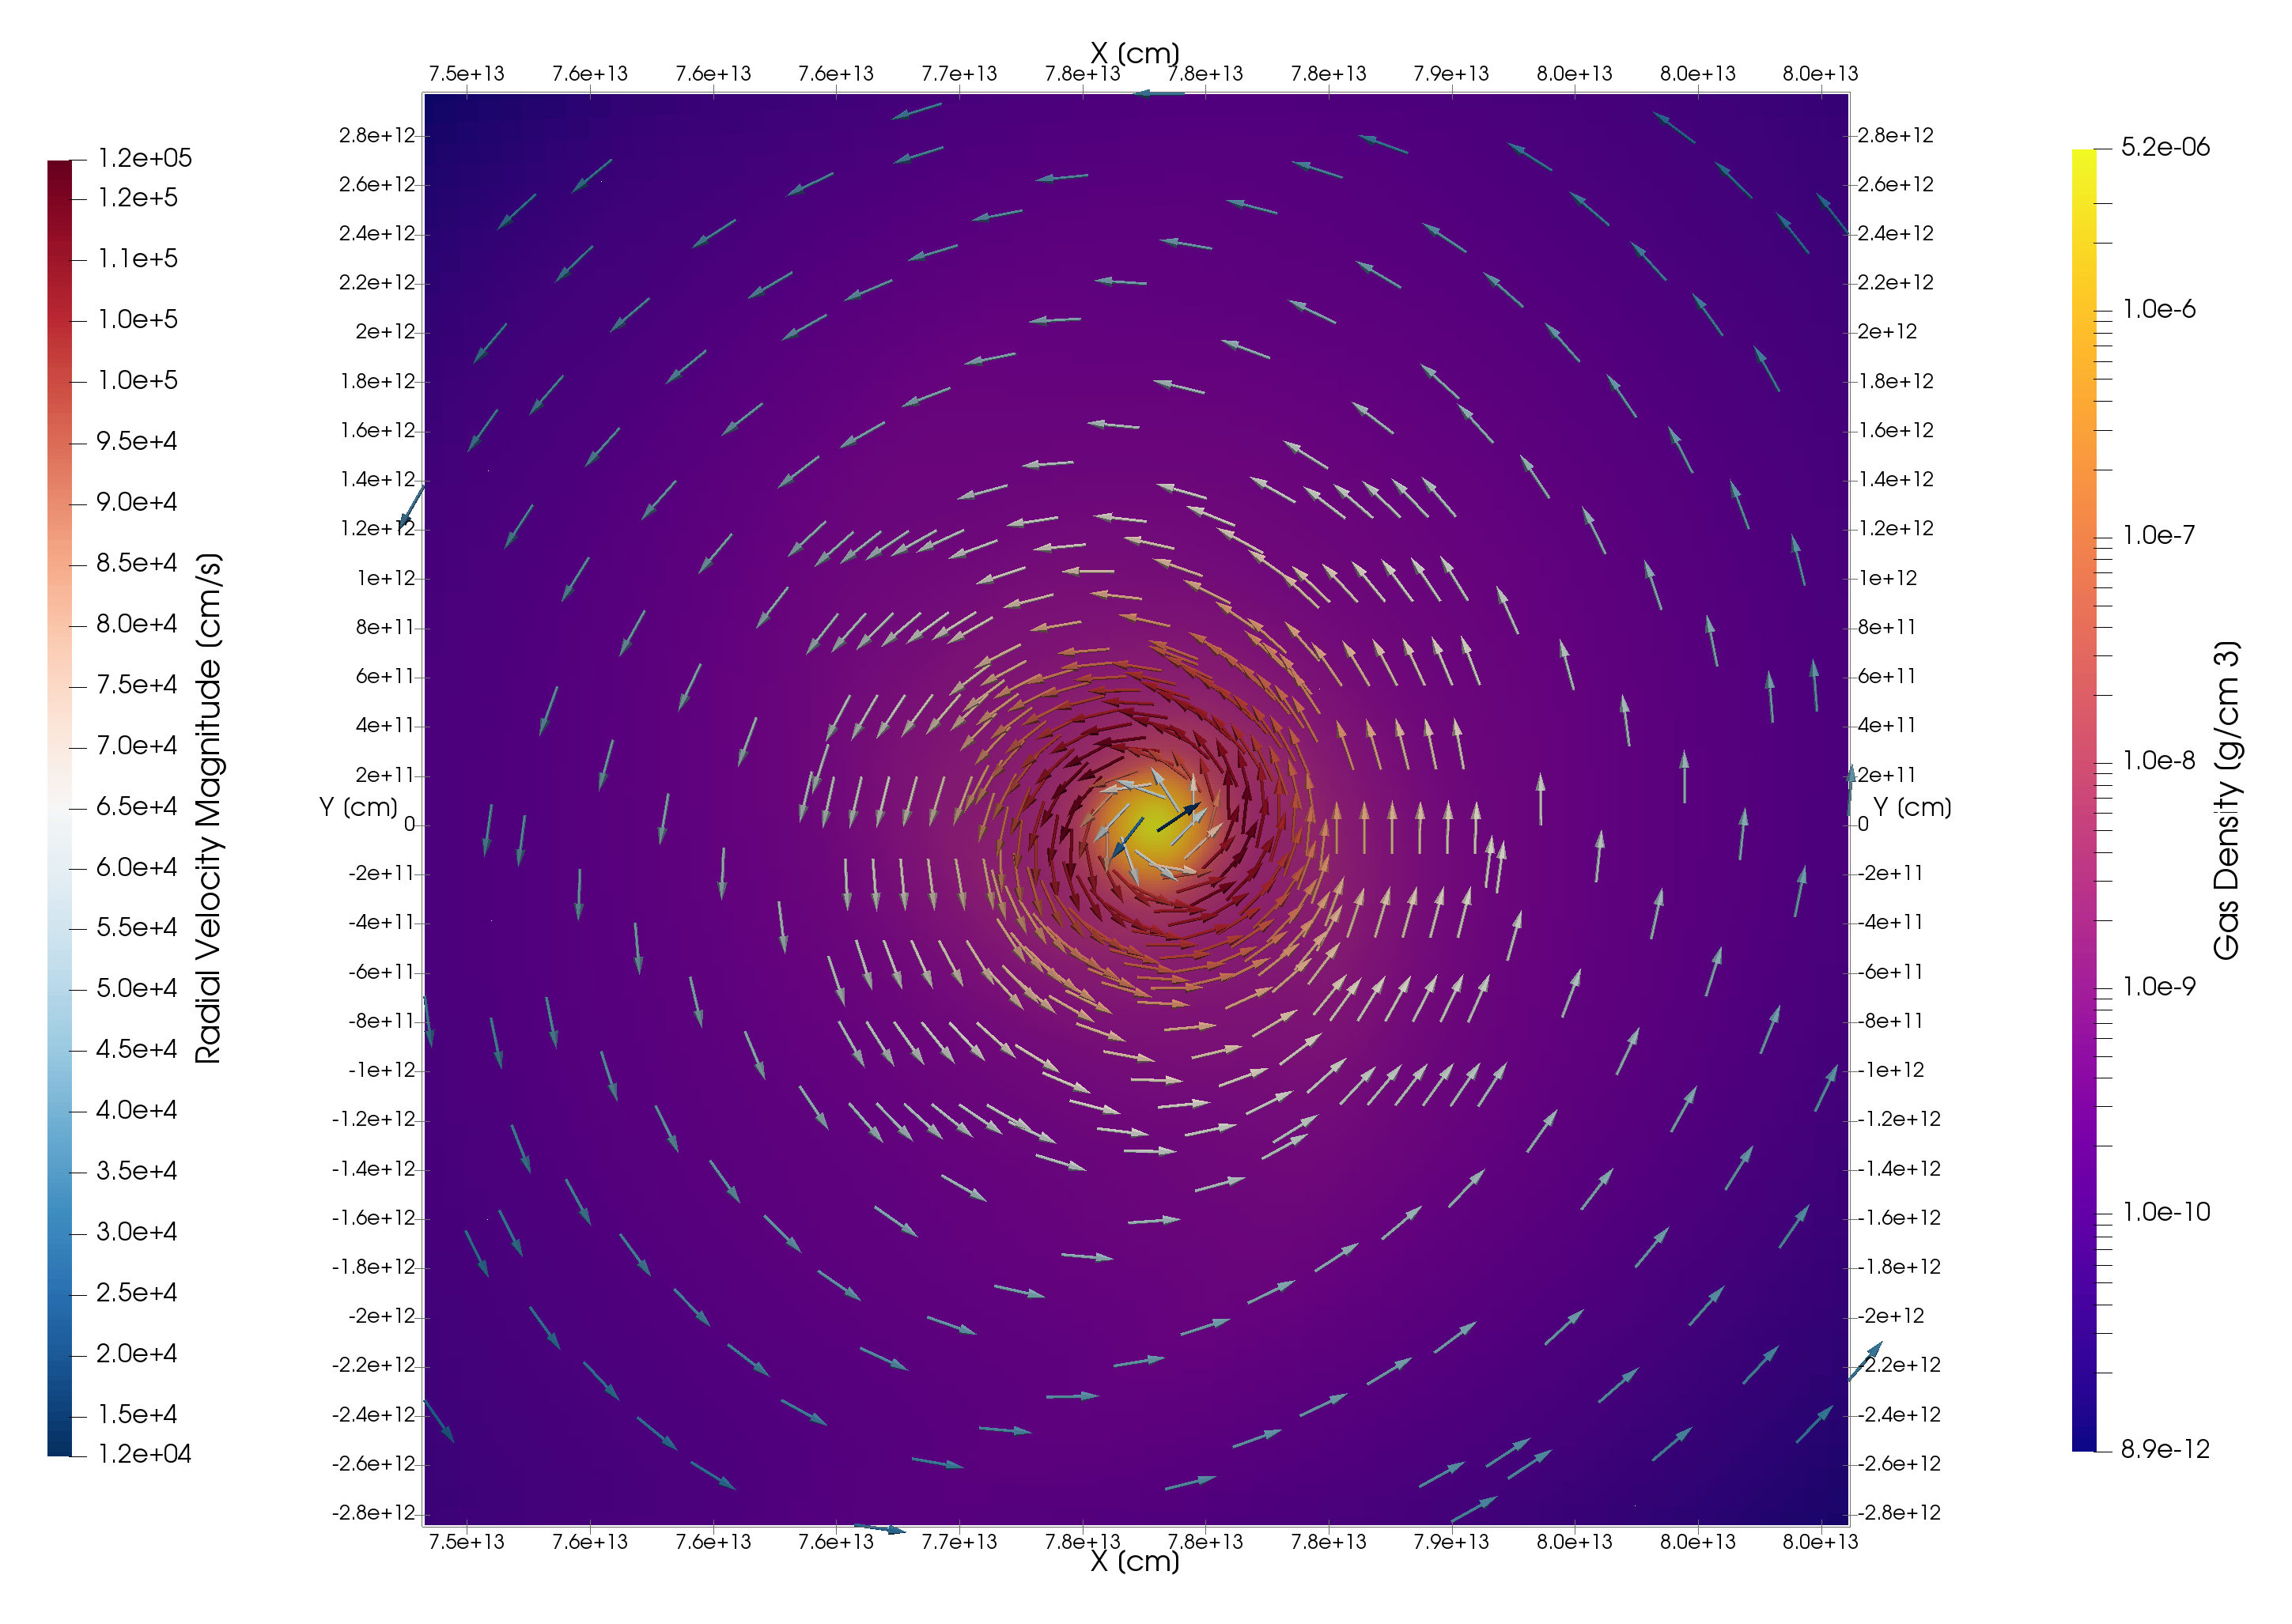
\includegraphics[width=0.95\linewidth]{figures/Presentation/OutFlowMidPlane.png}
	\caption{\label{fig:ofmid} Radial outflow of gas through the CPD, planet mass is 1 M${_J}$ located at 5.2AU.}
\end{figure}
\subsubsection{Circumplanetary disk flow}

During planet formation, the planet attracts gas and dust from the local environment. The JUPITER simulations show that this flow of material towards the planet is primarily from the vertical directions, Fig. \ref{fig:vel}. Gas from the edges of the gap where the CPD is embedded flows accelerates vertically towards accreting planet. As the gas in the region of the planet is adiabatically compressed, it heats up and forms a high pressure region surrounding the planet. The inflowing gas shocks on the upper boundary of the CPD near this region, forming a high temperature discontinuity, and losing most of its velocity Fig. \ref{fig:tshock}. Some of the material is then accreted onto the planet, while the majority flows outward in the CPD, Fig. \ref{fig:ofmid}, before being recycled into the circumstellar disk, Fig. \ref{fig:recirc}. The strength of this shock, along with the sharpness of the density discontinuity of the CPD and the gap in general will vary with both the planet mass and initial temperature. An exploration of the structure of CPDs can be found in \cite{Szulagyi2016}.
 
\renewcommand{\topfraction}{1}
\renewcommand{\bottomfraction}{1}

\begin{figure*}[htb!]
	\centering
	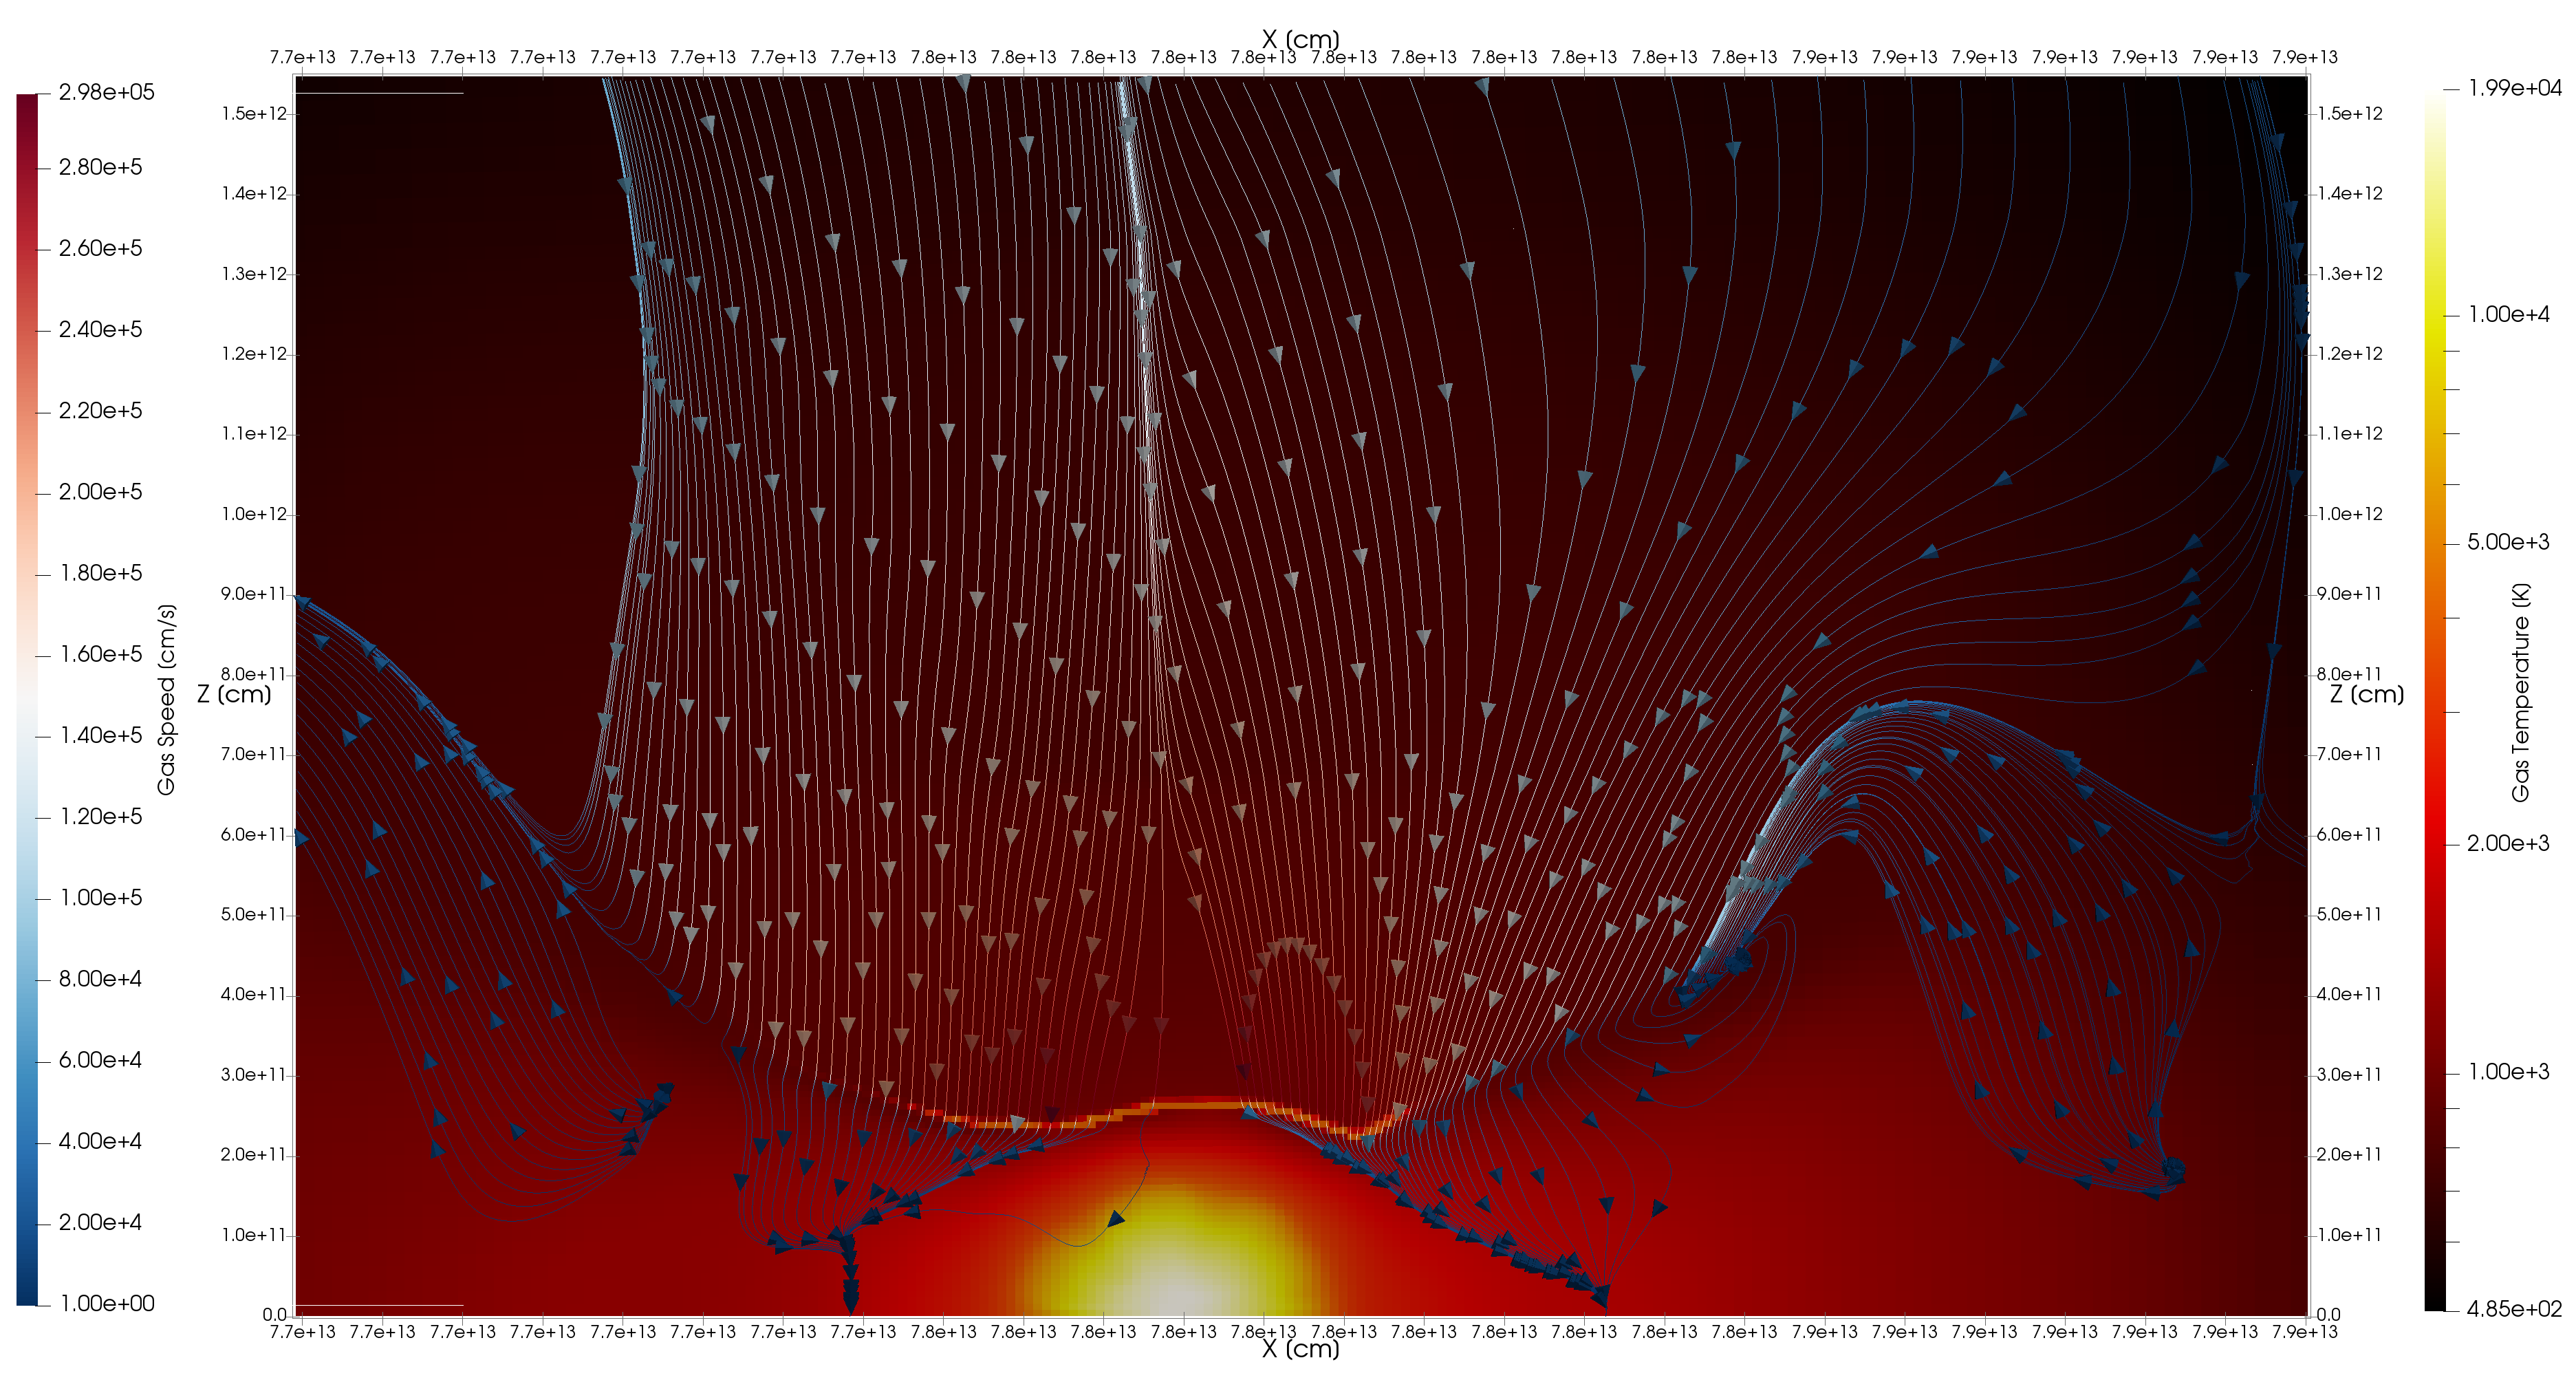
\includegraphics[width=0.95\linewidth]{figures/Presentation/GasShock.png}
	\caption{\label{fig:tshock} High temperature shock near the surface of the accreting 1 M$_{J}$ planet. After shocking upper boundary of the CPD, the inflowing gas loses some of its energy and spirals out in the CPD.}
\end{figure*}

\subsubsection{Dust traps and implications for satellite formation}

Visible in Figs.  \ref{fig:vel} and \ref{fig:tshock}, there are regions where inflowing gas from the circumstellar disk and outflowing gas from the CPD meet.
Inflowing gas from the gap walls flows over this high pressure region and the CPD, forming a vortex at approximately 20 planet radii from the planet. This forms a circular ring that acts as a dust trap, providing an ideal location for satellite formation.  According to \cite{satellite}, the dust-to-gas ratio in the dust trap can increase to 1 or greater. While beyond the scope of this report to analyse this phenomena in detail, it is discussed at length in \cite{satellite}.

\subsubsection{Gap profiles}

In addition to the flow analysis, we can also examine the gap properties that arise from planet-disk interactions. 
In Fig. \ref{fig:gaps}, we see that both the gap widths and gap depths increase as the planet mass increases. Comparing the 1 M$_{J}$ simulation to the 10 M$_{J}$, the gap width increases by a factor of 2 while the depth decreases from 8$\times10^{-16}$g cm$^{-3}$ to 5$\times10^{-20}$g cm$^{-3}$. Additional structure such as spiral arms or gap asymmetries also become more visible in the density profile of the disk as the planet mass increases. 

However, these properties are also highly dependant on the radial position of the planet, and are also highly viscosity dependant. Other studies have shown that planetary properties can be derived from observed disk features.

%\begin{figure}
%	\centering
%	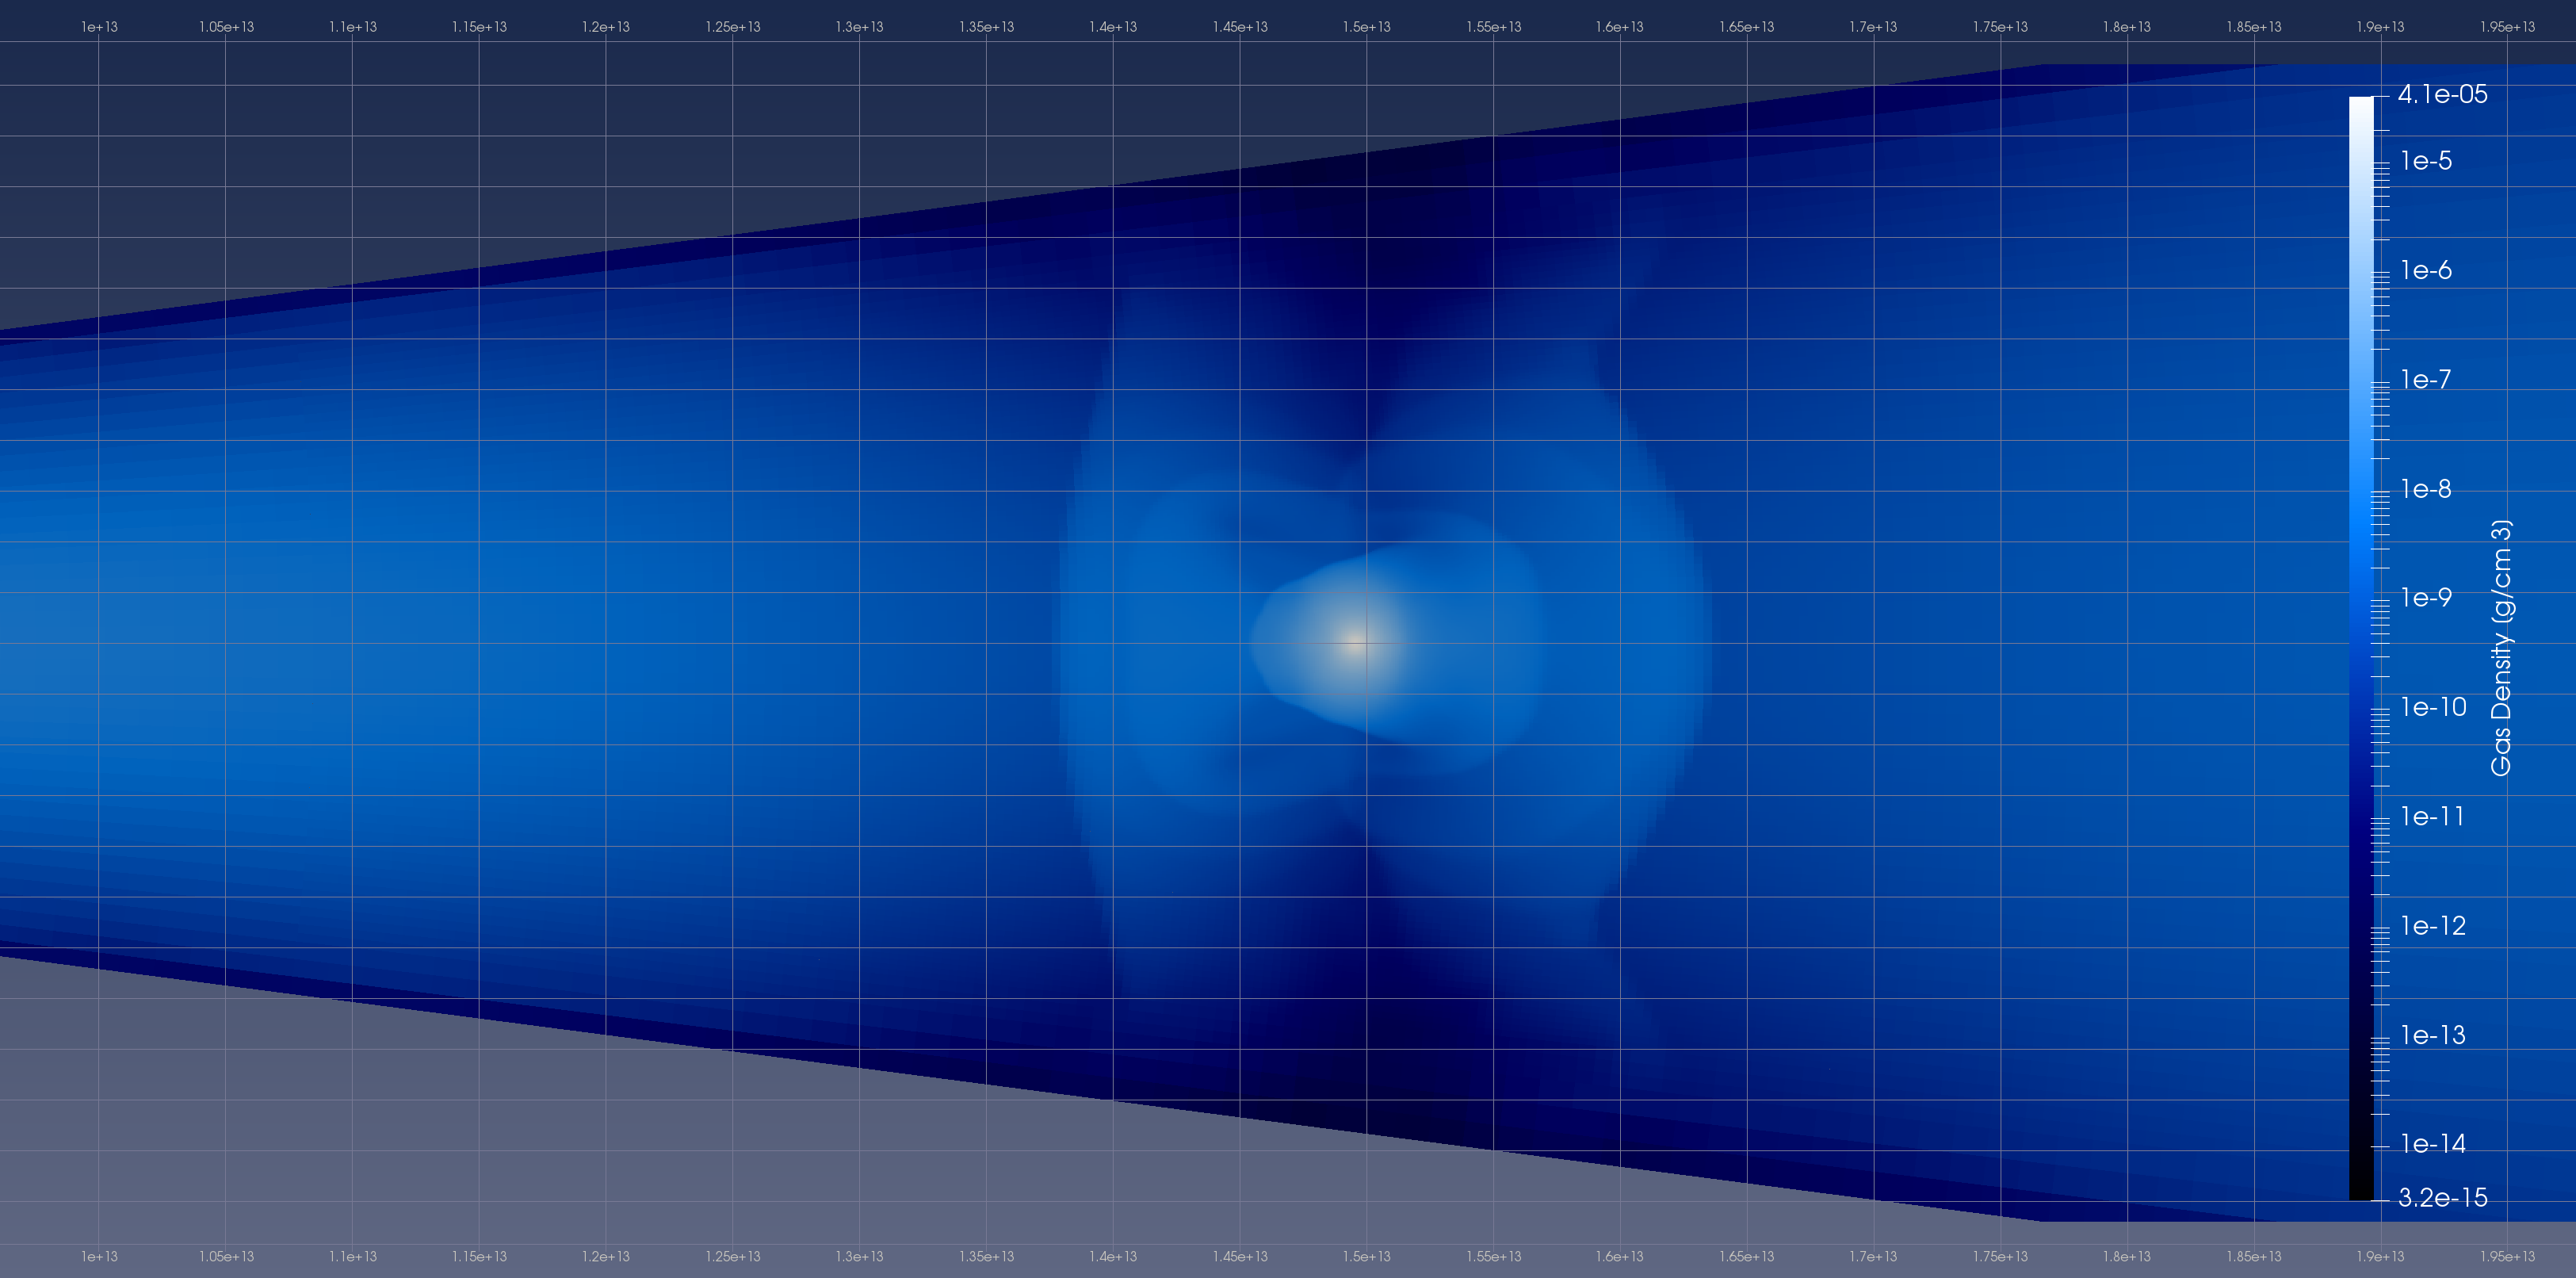
\includegraphics[width=\linewidth]{figures/DensWithGrid.png}
%	\caption{\label{fig:dens} Example of the 3D density structure of the circumplanetary disk as rendered in Paraview.}
%\end{figure}
%\begin{figure}
%	\centering
%	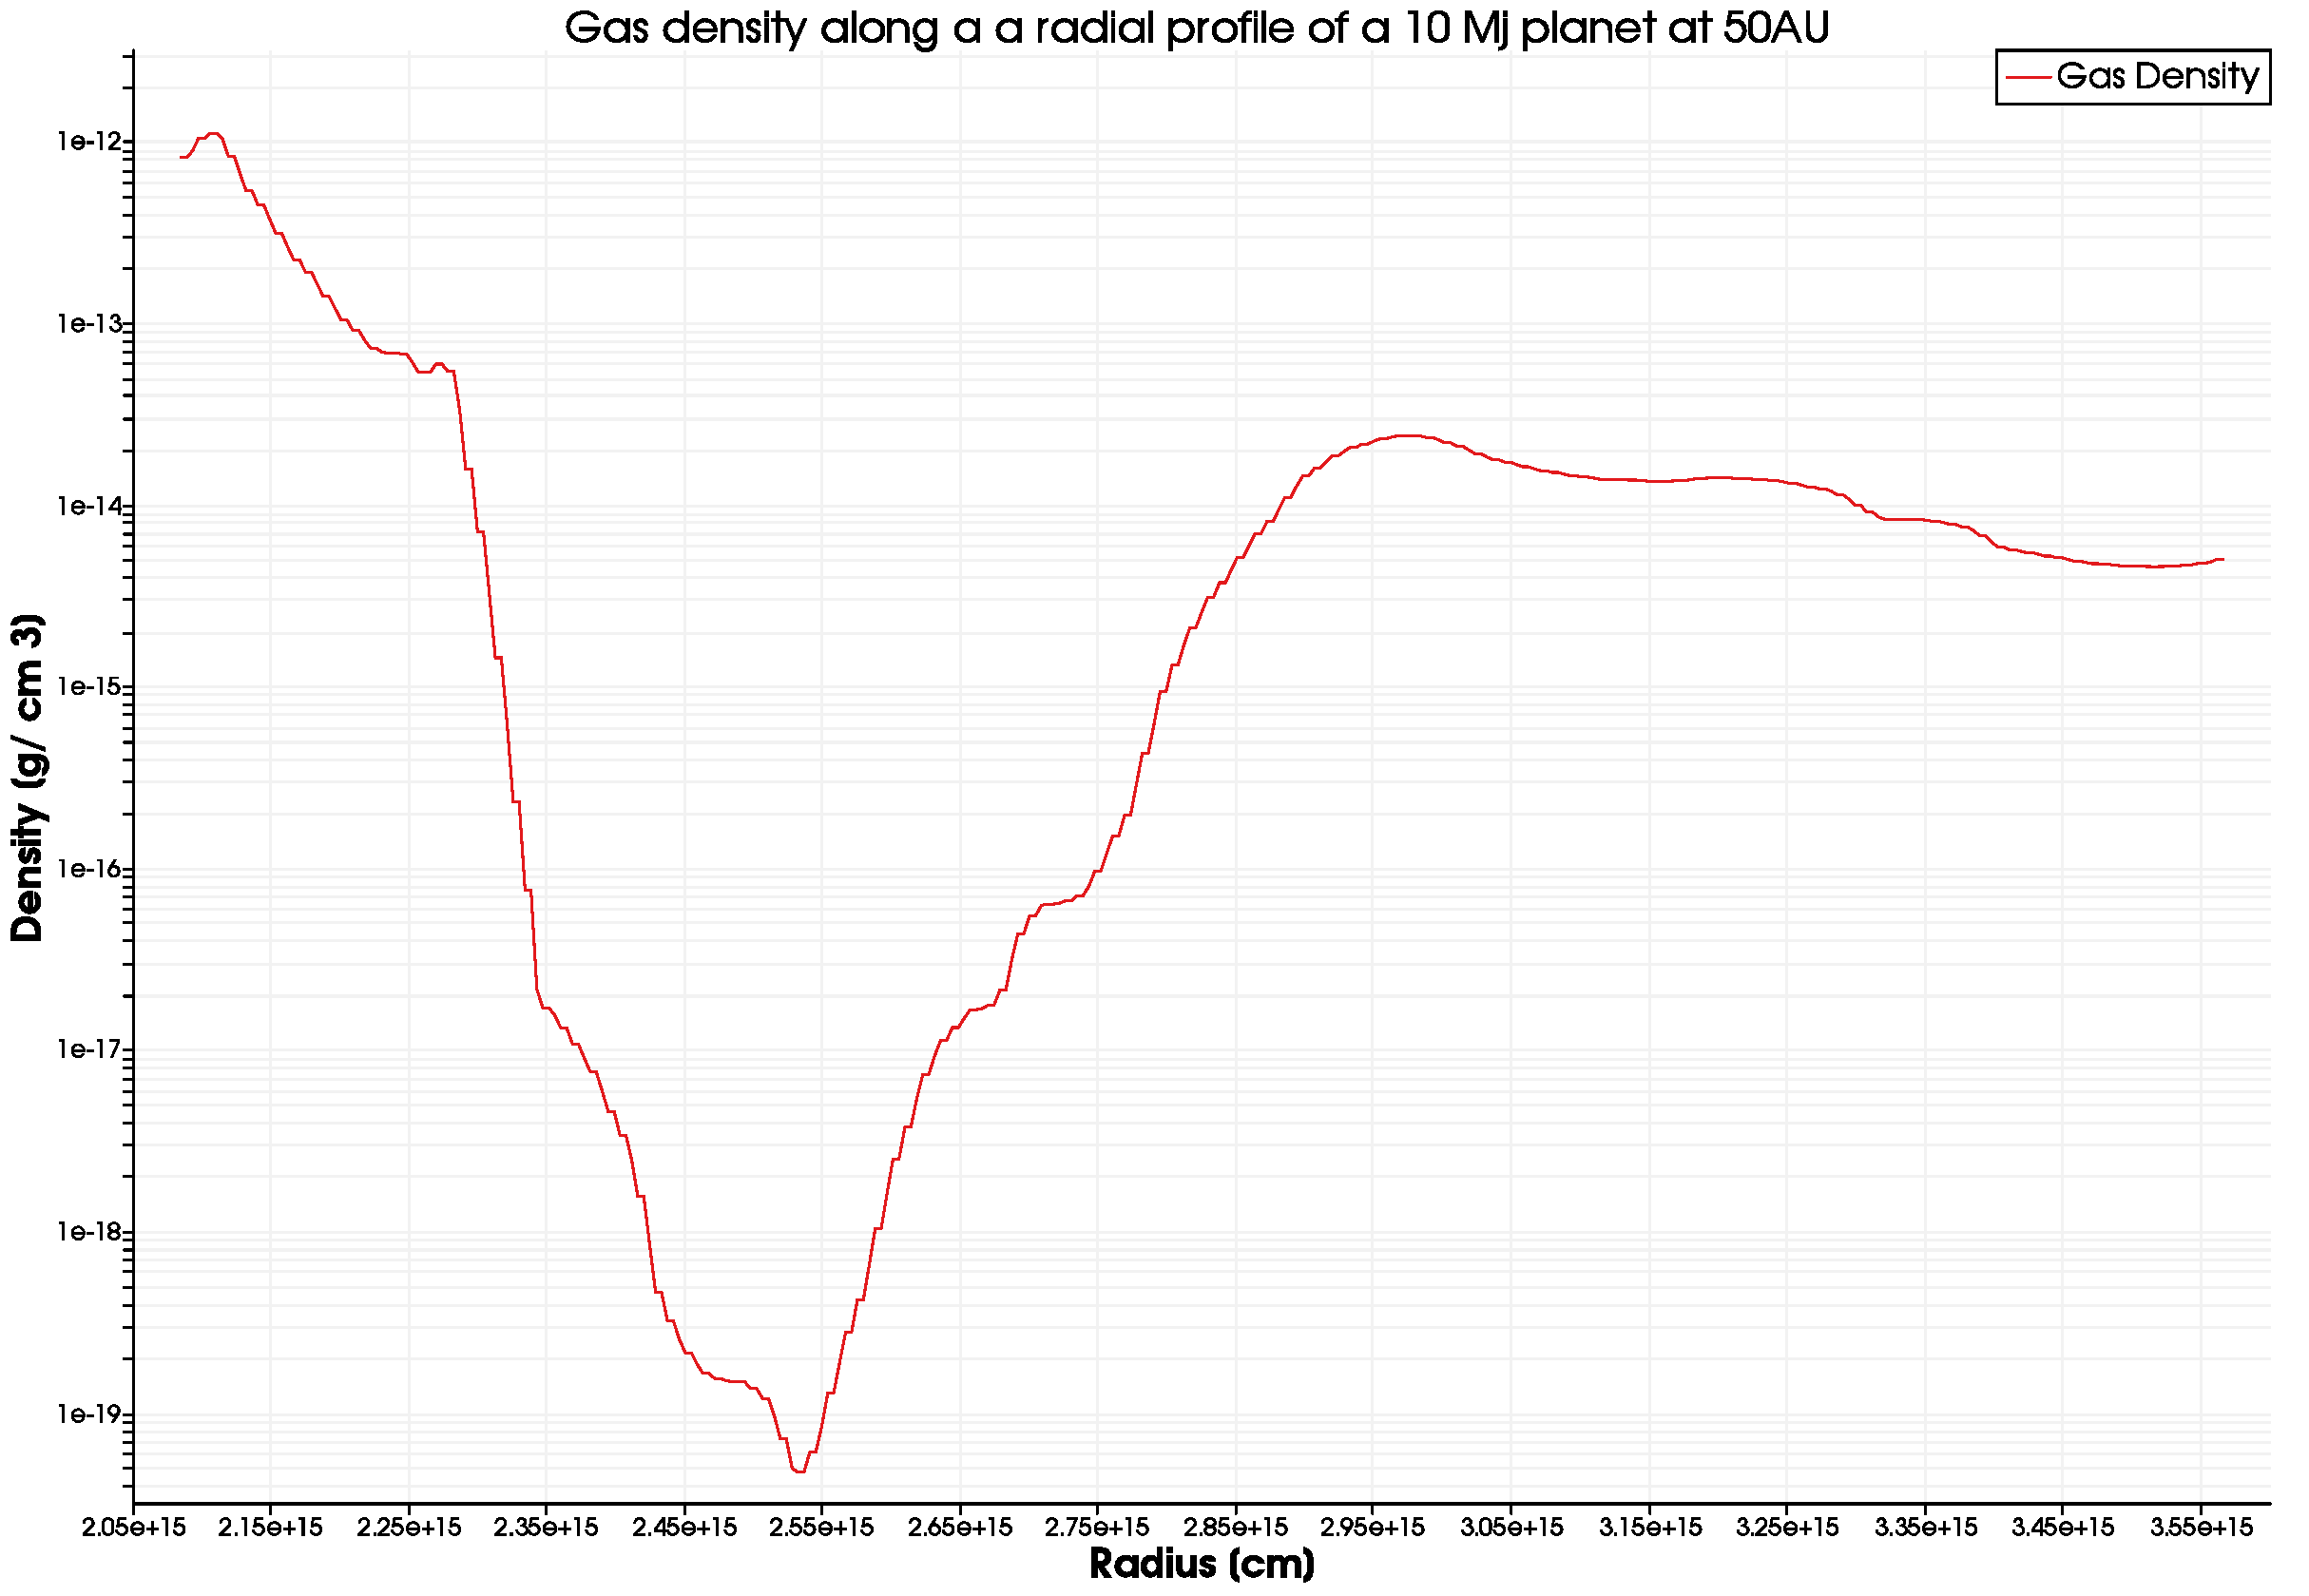
\includegraphics[width=\linewidth]{figures/Presentation/Gaps/radprof.pdf}
%	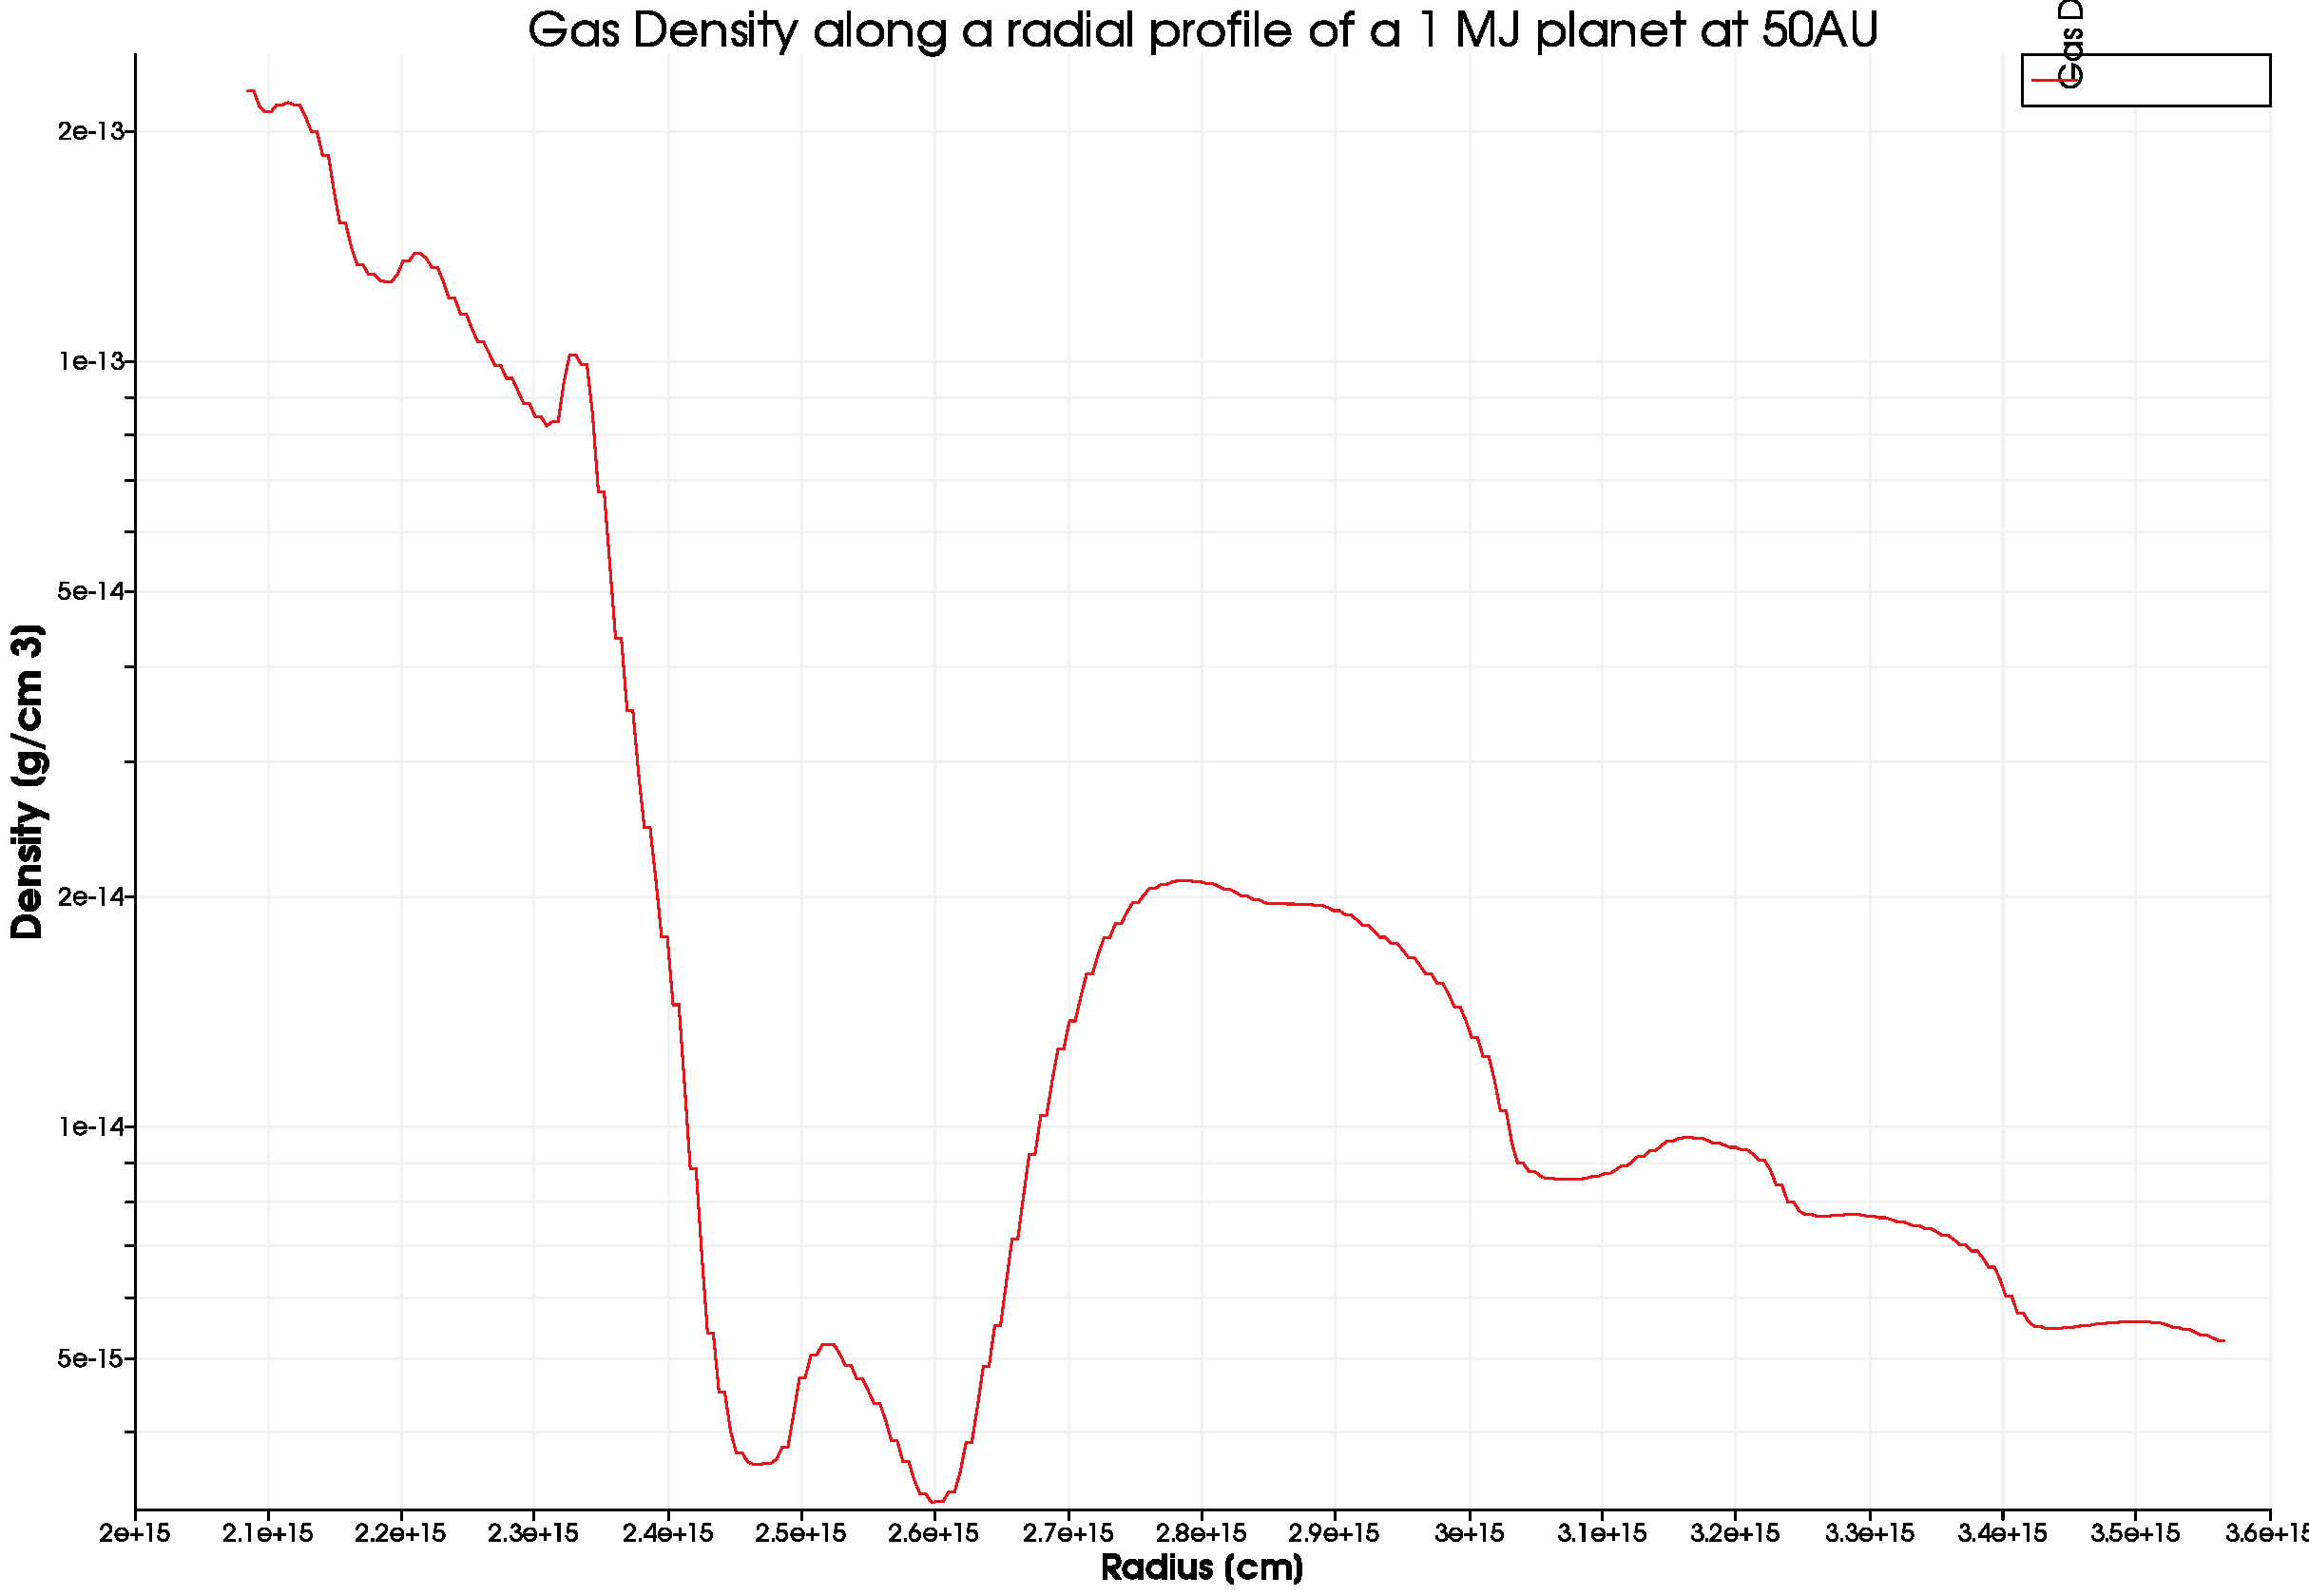
\includegraphics[width=\linewidth]{figures/Presentation/Gaps/radprof_1mj.pdf}
%	\caption{\label{fig:densrad} Example of the 3D density structure of the circumplanetary disk as rendered in Paraview.}
%\end{figure}
% Fig. \ref{fig:dens} shows a cross section of the gas density in the region of the circumplanetary disk along with the 3D density structure in Fig. \ref{fig:d3d}. This shows the dens regions near to the forming planet, and a potential location for satellite formation. Fig. \ref{fig:temp} shows the gas temperature of the mid-plane of the disk, coloured to a blackbody spectrum.

%Fig. \ref{fig:vel} shows the gas velocity in the circumplanetary disk, showing that the gas is spiralling away from the planet. This demonstrates that the circumplanetary disk is \textit{not} an accretion disk, but rather a de-accretion disk, as gas that flows in from above and below the planet spirals away in the disk. This flow is also shown in Fig. \ref{fig:tube}. In addition, Fig. \ref{fig:shock} shows the location in the temperature profile where the infowing gas shocks as it approaches the dense planet. Fig. \ref{ref:energy} shows the increase in internal energy of the gas near the planet as it is adiabatically compressed.

%More complicated renders -- particularly when rendering 3D volumes -- are very computationally expensive, and it is recommended to set up a Paraview server dedicated to rendering the dataset.
%Other possibilities include 3D time series animates, image generation using python scripts, streamline and flow visualisation and more.

\section{Conclusions}\label{sec:con}
We have successfully developed a data processing tool to allow JUPITER simulations results to be visualised using Paraview or other VTK software. This will allow further exploration of the physics of circumstellar and circumplanetary disks, as the increasingly complex 3D results require adequate visualisation to understand and study. 

Various visualisation and analysis techniques have been examined, including Paraview, Python VTK and matplotlib. 
Each tool has its own strengths and weaknesses, and the choice of visualisation tool should depend on the desired outcome.

In general, we recommend the use of Paraview both as an exploratory tool to examine 3 dimensional data, but also to produce high quality renders. 
Python VTK is useful for the generation of simple, repetitive plots from a consistent dataset, and allows for a degree of automation. 
Finally, matplotlib should be used to generate plots that maintain a consistent aesthetic with other figures in scientific works.

We also present a qualitative analysis of several simulations. 
We note the flow patterns in 3 dimensional simulations are inconsistent with traditional 1D planet formation models, but may represent a more realistic scenario of gas flow.
We also demonstrate that planet properties will have an effect on the observational properties of protoplanetary disks, though the derivation of planetary properties from disk features is not a subject of this report.

\section{Acknowledgements}
I would like to sincerely thank my supervisor Dr. Judit Szul\'{a}gyi for her guidance, mentorship and patience during this project.

Thanks as well to Prof. Hans Martin Schmid for allowing me to be a part of the Star and Planet Formation group at ETH Z\"{u}rich.

I would also like to acknowledge the Kitware Inc. for supporting the open source platforms of the Visualization ToolKit (VTK)  and Paraview, upon which this work relies.


%% This command is needed to show the entire author+affilation list when
%% the collaboration and author truncation commands are used.  It has to
%% go at the end of the manuscript.
%\allauthors

%% Include this line if you are using the \added, \replaced, \deleted
%% commands to see a summary list of all changes at the end of the article.
%\listofchanges
%% The reference list follows the main body and any appendices.
%% Use LaTeX's thebibliography environment to mark up your reference list.
%% Note \begin{thebibliography} is followed by an empty set of
%% curly braces.  If you forget this, LaTeX will generate the error
%% "Perhaps a missing \item?".
%%
%% thebibliography produces citations in the text using \bibitem-\cite
%% cross-referencing. Each reference is preceded by a
%% \bibitem command that defines in curly braces the KEY that corresponds
%% to the KEY in the \cite commands (see the first section above).
%% Make sure that you provide a unique KEY for every \bibitem or else the
%% paper will not LaTeX. The square brackets should contain
%% the citation text that LaTeX will insert in
%% place of the \cite commands.

%% We have used macros to produce journal name abbreviations.
%% \aastex provides a number of these for the more frequently-cited journals.
%% See the Author Guide for a list of them.

%% Note that the style of the \bibitem labels (in []) is slightly
%% different from previous examples.  The natbib system solves a host
%% of citation expression problems, but it is necessary to clearly
%% delimit the year from the author name used in the citation.
%% See the natbib documentation for more details and options.
\bibpunct{(}{)}{;}{a}{}{,} % to follow the A&A style
\bibliographystyle{aasjournal}
\bibliography{biblio.bib}

\begin{appendix}
	\section{Legacy VTK File Format}
	An example of a simple VTK file \cite{Formats2009}:
	\begin{lstlisting}
	# vtk DataFile Version 2.0
	Jupiter Simulation Data
	ASCII
	DATASET UNSTRUCTURED_GRID
	POINTS n double
	p$_{0x}$ p$_{0y}$ p$_{0z}$
	...
	p$_{(n-1)x}$ p$_{(n-1)y}$ p$_{(n-1)z}$
	
	CELLS m 
	nVert$_{0}$ i0 i1 i2 ... i(nVert$_{0}$-1)
	...
	nVert$_{(m-1)}$ i0 i1 i2 ... i(nVert$_{(m-1)}$-1)
	
	CELL_TYPE m 
	type$_{0}$
	..
	type$_{(m-1)}$
	
	CELL_DATA m
	SCALARS name double
	LOOKUP_TABLE default
	s$_{0}$
	...
	s$_{(m-1)}$
	\end{lstlisting}
\end{appendix}
\end{document}

% End of file `sample62.tex'.
